\documentclass[a4paper,%
				12pt,%
				oneside%
				]{book}
				
\usepackage[english,italian]{babel}

%\usepackage[T1]{fontenc} % Riga da togliere se si compila con PDFLaTeX
\usepackage[utf8]{inputenc} % Consente l'uso caratteri accentati italiani
\usepackage{graphicx}
\usepackage{fancyhdr}
\usepackage{setspace}
\usepackage{subfig}
\usepackage{caption}
\usepackage[backend=bibtex]{biblatex}

\bibliography{Bibliografia}


\graphicspath{{./Immagini_fake/}}

\nocite{*}

\setcounter{secnumdepth}{3}
\setcounter{tocdepth}{2}

\frenchspacing % forza LaTeX ad una spaziatura non inglese
\hoffset + 0.5cm

\renewcommand{\sectionmark}[1]{%
\markboth{\MakeUppercase{%
\thesection. \ #1}}{}}


\rhead{\thesection \sectionmark}
%\lhead{}
\lfoot{}%\emph{Francesco Capozzo}}
\cfoot{\thepage}
\rfoot{}
\renewcommand{\headrulewidth}{0.4pt}
\renewcommand{\footrulewidth}{0.4pt}


\renewcommand{\contentsname}{Sommario}
\renewcommand{\listfigurename}{List of Figures}
\renewcommand{\listtablename}{List of Tables}
\renewcommand{\bibname}{Bibliografia}
\renewcommand{\indexname}{Indice}
\renewcommand{\figurename}{Figura}
\renewcommand{\tablename}{Tavola}
\renewcommand{\partname}{Parte}
\renewcommand{\chaptername}{Capitolo}
\renewcommand{\appendixname}{Appendice}
\renewcommand{\today}{\ifcase\month\or
  Gennaio\or Febbraio\or Marzo\or Aprile\or Maggio\or Giugno\or
  Luglio\or Agosto\or Settembre\or Ottobre\or Novembre\or Dicembre\fi
  \space\number\day, \number\year}
  
  
%riduce lo split delle footnote
\interfootnotelinepenalty=10000


\newtheorem{thm}{Teorema}

\theoremstyle{definition}
\newtheorem{defn}{Definizione}


\floatstyle{boxed}
%\newfloat{program}{thp}{lop}[chapter]
\newfloat{program}{tbphH}{lop}[chapter]
\floatname{program}{Codice}

\newcommand{\codefrom}[2][CLIPS]
{
\begin{program}[p]
    \lstinputlisting[language=#1]{#2}
    \caption{#2}
    \label{#2}
\end{program}
}

%\newenvironment{program}{\begin{boxedverbatim}}{\end{boxedverbatim}}


% Vincoli

% Initializing the counters and define a custom label
\newcommand{\vincoliinit}{
    % Create a new counter for keeping track of the last number
    \newcounter{vincolicountbackup}
    % Create a new counter for the custom label
    \newcounter{vincolicount}
    % Redefine the command for the last counter so when it is called
    % it prints the number like this in a bold font: R<number>
    \renewcommand{\thevincolicount}{\textbf{Vincolo-\arabic{vincolicount}: }}
}

% Used to define the start of the requirements
\newcommand{\vincolistart}{
    % Indicate the start of a new list and tell it to use the redefined
    % command and corresponding counter for every item
    \begin{list}{\thevincolicount}{\usecounter{vincolicount}}
    % Important part: set the value of the used counter to the
    % same value of the backup counter.
    \setcounter{vincolicount}{\value{vincolicountbackup}}
}

% Used to define the end of the requirements
\newcommand{\vincoliend}{
    % Important part: take the value of the used counter (after
    % being incremented by the requirement items) and store it
    % in the backup counter.
    \setcounter{vincolicountbackup}{\value{vincolicount}}
    % Mark the end of the list environment
    \end{list}
}


% COLORI

\definecolor{grigio-chiarissimo}{rgb}{0.9,0.9,0.9}


% grafici

%\pgfplotsset{/pgf/number format/use comma,compat=newest}

\lstset{%
	basicstyle=\footnotesize\ttfamily,
	frame=single,
	captionpos=b,
	breaklines=true,
	tabsize=2,
	numbers=left
}

\renewcommand{\lstlistingname}{Codice}                  % file con le impostazioni personali

				
\begin{document}

\pagenumbering{roman}
\pagestyle{plain}

% !TEX root = ../Tesi.tex

\begin{center}

\includegraphics[height=2cm]{Immagini/logo.png}\\
\LARGE{UNIVERSITA' DEGLI STUDI DI BARI}\\
%\Huge{\textbf{ALDO MORO}}\\
\LARGE{ALDO MORO}\\
\vspace{0.5cm}
\small{FACOLTA' DI SCIENZE MATEMATICHE, FISICHE E NATURALI}\\
CORSO DI LAUREA IN\\
INFORMATICA\\
\hrulefill \\ %liena oritizontale
\vspace{0.2cm}
TESI DI LAUREA\\
\vspace{0.2cm}
IN\\
\vspace{0.2cm}
\normalsize{INGEGNERIA DELLA CONOSCENZA E SISTEMI ESPERTI}\\
\vspace{2cm}%inserisci una riga vuota(spazio rigido 
\large{\textbf{.\ .\ .\ }}\\
\thispagestyle{empty}%per non numerare la prima pagina
\end{center}
\vspace{3cm}
RELATORI:\\
Chiar.ma Prof.ssa Floriana Esposito\\
Chiar.mo Prof Stefano Ferilli

\begin{flushright}
LAUREANDO:\\
Francesco Capozzo\\
\end{flushright}
\hrulefill
\begin{center}
\small{ANNO ACCADEMICO 2011/2012}
\end{center}

\pagestyle{fancy}

 

\tableofcontents % Prepara l'indice generale
\listoffigures
\listoftables

 

\mainmatter
\chapter{Environment per Sistemi Esperti}

\setcounter{section}{1}
\phantomsection\addcontentsline{toc}{section}{\protect\numberline{\thesection}Sistemi Esperti}
\sectionmark{Sistemi Esperti}

\begin{quote}
''Un esperto è una persona alla quale, per motivi professionali o per una acquisita competenza ed esperienza su una data materia, viene richiesto di fornire pareri scientifici su argomenti di dettaglio.'' (Wikipedia)
\end{quote}

Sembra ragionevole la scelta di attribuire l'aggettivo di \emph{esperto} a una persona in possesso di qualità e caratteristiche che ne attestino una conoscenza in uno specifico ambito di dominio e che sia in grado di risolvere direttamente problemi o fornire possibili soluzioni in seguito ad una attività di ragionamento.
Realizzando un parallelismo, è possibile considerare l'assegnazione dell'attributo di \emph{esperto} ad un sistema in grado di esibire un comportamento paragonabile a quello di un esperto umano all'interno di un ambito di dominio focalizzato.
La definizione fornita in \cite{jackson1999} spiega il \emph{sistema esperto} come un'applicazione che rappresenta e ragiona con conoscenza di tipo specialistico con l'obiettivo di risolvere problematiche o fornire consigli su come risolverle.

L'obiettivo di utilizzo di un \emph{sistema esperto} può essere quello di sostituire completamente l'intervento umano durante lo svolgimento di un'attività o di fornire supporto ad un esperto durante l'atto di prendere una decisione, giocando un ruolo di assistenza. Altre possibili applicazioni possono riguardare la formazione o il perfezionamento della conoscenza posseduta da un esperto tramite l'interazione diretta con il sistema a titolo di confronto o consultazione.

I sistemi esperti sono applicazioni progettate per rendere disponibili alcune abilità di esperti di un dominio anche a utenti non esperti. Siccome questo genere di programmi tentano di emulare gli schemi mentali e i modi di pensare di un esperto, è naturale che le prime ricerche in questo ambito siano state effettuate nel campo dell'\emph{intelligenza artificiale}: una branca delle Scienze Informatiche correlate con la progettazione e la realizzazione di applicazioni in grado di emulare le abilità cognitive umane nel campo della soluzione di problemi, la percezione e la comprensione del linguaggio~\cite{feigenbaum1981ia}.

Ciò che differenzia un'applicazione convenzionale da un \emph{sistema esperto} può essere sintetizzato in tre caratteristiche fondamentali: perché ragiona; su cosa ragiona; come ragiona.

L'obiettivo di un sistema esperto è quello di simulare un ragionamento umano nell'ambito di un dominio, piuttosto che simulare il dominio stesso. Le applicazioni convenzionali lavorano attraverso la realizzazione di un modello matematico al fine simulare le abilità dell'esperto nella soluzione del problema. I sistemi esperti invece focalizzano l'attenzione sull'emulazione degli schemi di ragionamento che l'esperto adotta per ottenere delle soluzioni e tentano di emulare il processo di ragionamento e non semplicemente il risultato allo specifico problema.

Un altro fattore discriminante riguarda il tipo di informazioni sulle quali i due sistemi lavorano: le applicazioni tradizionali utilizzano modelli per rappresentare il problema, applicano algoritmi per la manipolazione dei dati ed infine calcolano soluzioni. Nei sistemi esperti, invece, l'intero processo di ragionamento viene eseguito lavorando su rappresentazioni della conoscenza umana. Queste rappresentazioni vengono codificate utilizzando linguaggi specificamente sviluppati e che permettono di separare la rappresentazione della conoscenza di dominio dalle porzioni del sistema che invece rappresentano le dinamiche di ragionamento. Queste due porzioni dei sistemi esperti vengono definite con i nomi di \emph{base di conoscenza} e \emph{motore inferenziale}.

Le meccaniche di soluzione rappresentano l'ultimo fattore di differenza: se le applicazioni tradizionali risolvono problematiche offrendo soluzioni algoritmiche a problemi per i quali è stato individuato un modello, i sistemi esperti ottengono soluzioni applicando metodi approssimati o \emph{euristiche}\footnote{L’\emph{euristica} è una strategia cognitiva, una scorciatoia di pensiero, una tecnica basata su esperienze, che permette più rapidamente di elaborare giudizi, ricavare inferenze dal contesto, attribuire significato alle situazioni e prendere decisioni a fronte di problemi complessi o di informazioni incomplete~\cite{euristiche1}~\cite{kahneman1982judgment}.} spesso utilizzando conoscenza incerta o incompleta.

Proprio a causa della natura dinamica e incerta del ragionamento alla base dei \emph{sistemi esperti}, a questa classe di sistemi viene richiesta la capacità di interagire con l'utente (sia esso un esperto o no) in modo da:
\begin{itemize}
	\item illustrare e spiegare il ragionamento adottato per ottenere delle soluzioni e giustificare in questo modo il suo operato; 
	\item interagire con il mondo esterno tramite specifici protocolli, in modo da rendere possibile il reperimento di informazioni aggiuntive, qualora queste risultassero necessarie, durante il processo di ragionamento.
\end{itemize}

\begin{quotation}
''La \emph{vera} intelligenza richiede l'abilità di imparare, di ragionare sull'esperienza, d'agire d'istinto\footnote{L'espressione originale usava la forma gergale \emph{''to shoot from the hip''} la cui traduzione letterale rimanda al movimento dei cowboy di sparare velocemente dal fianco senza mirare con precisione.}, di usare conoscenza generale, di fare inferenza usando intuizioni \emph{viscerali}. I sistemi esperti non fanno niente di tutto ciò, Non migliorano i risultati sulla base dell'esperienza. Loro [i sistemi esperti] sanno soltanto spostarsi da una regola \emph{if/then} all'altra.'' \cite{schank1984ia} 
\end{quotation}

La capacità di apprendimento, che per Schank \cite{schank1984ia} è uno dei fattori determinanti per poter associare al ragionamento dei sistemi esperti l'attributo di \emph{intelligente}, rappresenta un'ulteriore componente chiave nella definizione di sistemi esperti. Alcune tecniche basate sull'aggiunta di nuovi elementi nella base di conoscenza o sull'aggiunta di nuove euristiche hanno permesso di integrare meccanismi di apprendimento automatico all'interno dei sistemi esperti~\cite{nasa1988flops}.

Dalla metà degli anni '60 ad oggi  sono stati creati un gran numero di sistemi esperti con ambiti di utilizzo molto differenti fra loro. Per fare alcuni esempi è possibile citare quello aerospaziale (ad esempio per agevolare alcune operazioni in orbita), quello sanitario (ad esempio nell'assistenza al monitoraggio dei parametri dei pazienti nelle unità di terapia intensiva o nella diagnosi di malattie) o quello finanziario.~\cite{jackson1999}

Il primi sistemi esperti prodotti furono Dendral (1965), con lo scopo di determinare la struttura molecolare partendo da dati provenienti da uno spettrometro di massa, R1 (1978), usato per configurare sistemi informatici e MYCIN (1976), per assistere nella diagnosi di infezioni da batteri e proporre piani terapeutici per il trattamento delle stesse.

\subsection{Le componenti di un sistema esperto} 

\begin{figure}[h]
\centering
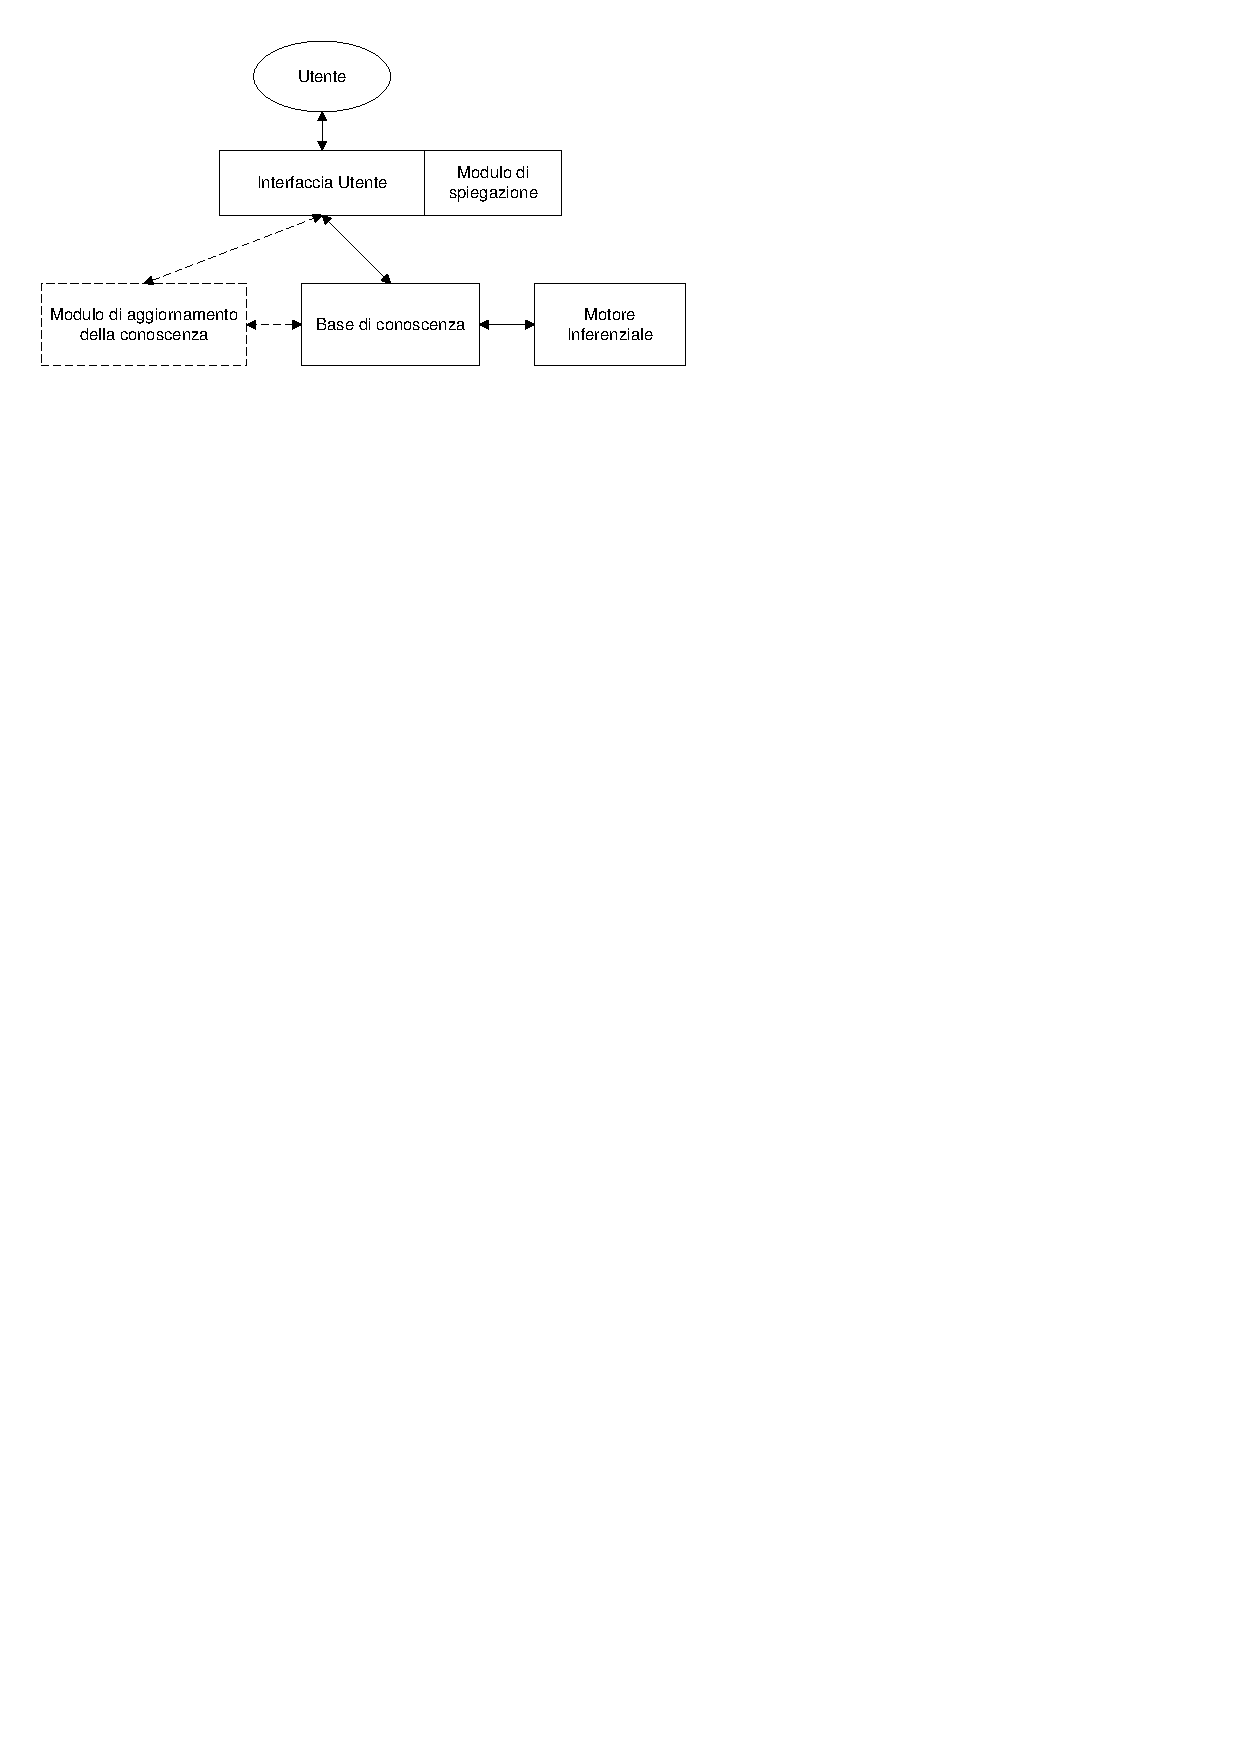
\includegraphics[viewport=19 667 329 824]{Immagini/Capitolo1/Architettura-SE.pdf}
\caption{Architettura semplificata di un generico Sistema Esperto}\label{fig:architettura-se}
\end{figure}

La struttura di un sistema esperto può essere sinteticamente descritta come composta da quattro moduli principali~(\figurename~\ref{fig:architettura-se}):
\begin{itemize}
	\item \emph{La base di conoscenza}: raccoglie tutta la conoscenza di dominio acquisita. La fonte principale d'informazione è rappresentata dall'esperto che, interrogato da un ingegnere della conoscenza, fornisce in maniera più o meno completa la conoscenza di cui dispone.
	\item \emph{Il motore inferenziale}: raccoglie i processi di ragionamento sulla base dei quali il sistema, usando congiuntamente la base di conoscenza e ulteriori (ed eventuali) informazioni ottenute dall'interazione diretta con l'utente, è in grado di dedurre nuove conoscenza.
	\item \emph{L'interfaccia utente}: permette l'interazione fra l'utente e il sistema. L'interazione può essere orientata verso la spiegazione del processo logico alla base di una soluzione o una scelta (attività svolta dal \emph{modulo di spiegazione}), oppure per ottenere ulteriori informazioni e far proseguire il ragionamento.
	\item \emph{Modulo di aggiornamento della conoscenza}: permette di modificare ed integrare quanto presente nella \emph{base di conoscenza} tramite processi automatici o che richiedono l'intervento di un esperto.
\end{itemize}

\subsection{Il processo di sviluppo di un sistema esperto}
Come il processo di sviluppo di software tradizionale può essere scandito in fasi e rappresentato all'interno dei vari modelli di sviluppo, anche la produzione di sistemi esperti può essere semplificata attraverso un modello suddiviso in step successivi. 

\begin{figure}[h]
\centering
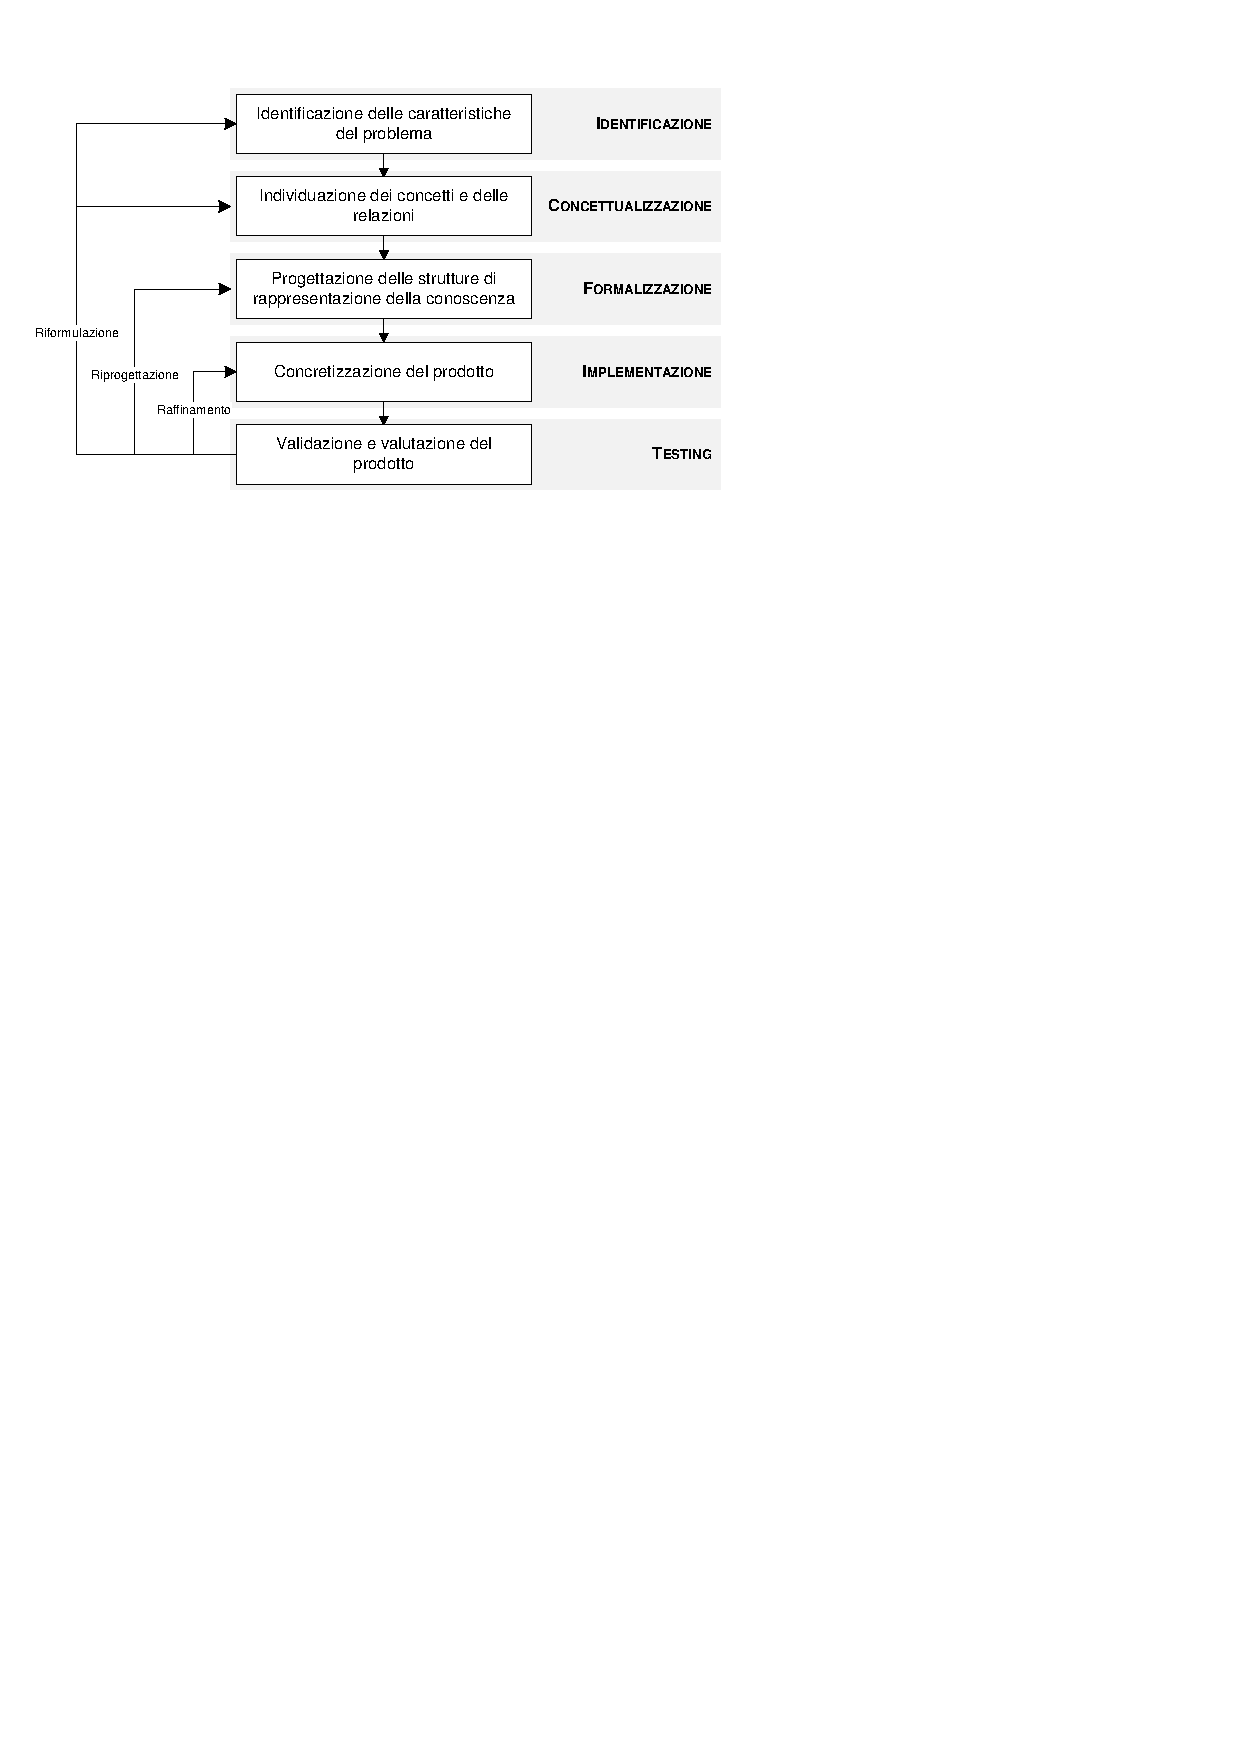
\includegraphics[viewport=16 607 346 801]{Immagini/Capitolo1/Fasi-acquisizione.pdf}
\caption{Le fasi di estrazione della conoscenza e sviluppo di un \emph{Sistema Esperto}}\label{fig:fasi-progettazione}
\end{figure}


Sebbene il confronto fra lo sviluppo di software tradizionale e quello di sistemi basati su conoscenza possa mostrare punti di contatto, le somiglianze sono solamente superficiali ed un'analisi approfondita rivelerebbe profonde differenze dettate dalle specifiche caratteristiche del tipo di artefatto in produzione.~\cite{esposito2012icse}

Alla figura già descritta dell'esperto di dominio viene affiancata quella dell'\emph{ingegnere della conoscenza}: un esperto informatico addetto alla compilazione di una base di conoscenza.

Come mostrato in \figurename~\ref{fig:fasi-progettazione} e suggerito in \cite{buchanan1983}, il processo può essere diviso in cinque fasi:
\begin{itemize}
	\item \emph{Identificazione}: è orientata all'identificazione della classe di problemi che il sistema dovrà risolvere, dei dati con i quali il sistema dovrà lavorare e dei criteri che le soluzioni dovranno soddisfare.
	
	\item \emph{Concettualizzazione}: ha la finalità di scoprire i concetti chiave e le relazioni che intercorrono fra loro. Questa fase dovrebbe includere la caratterizzazione delle varie tipologie di dati, il flusso delle informazioni e la delineazione delle strutture del dominio del problema.
	
	\item \emph{Formalizzazione}: le conoscenze e le relazioni fra le entità individuate ed organizzate nelle fasi precedenti vengono concretizzate tramite l'uso di un formalismo concordato dai membri appartenenti al team di sviluppo del sistema. In questa fase vengono eseguite le scelte relative alla tipologia di rappresentazione della conoscenza da adottare e gli strumenti da adoperare.
	\item \emph{Implementazione}: gli elementi ottenuti nei passi precedenti vengono convertiti in un artefatto completo.
	\item \emph{Testing}: l'artefatto viene sottoposto alla valutazione dell'esperto di dominio. Ne vengono valutate l'utilità e le prestazioni e verificata la corrispondenza con i requisiti fissati nelle fasi precedenti. In questa fase viene infine valutata la possibilità apportare modifiche, correggere difetti o integrare nuovi elementi nella strategia di controllo o nella base di conoscenza.
\end{itemize}

Il processo di acquisizione della conoscenza e sviluppo del sistema, sebbene possa sembrare rigoroso, non è affatto un processo lineare. Ad ogni fase viene associata un'attività di verifica e raffinamento eseguita tramite la consultazione dell'esperto di dominio.

L'attività di estrazione della conoscenza eseguita nelle fasi iniziali dello sviluppo non è un processo accurato o esente da errori: durante le interviste condotte dagli ingegneri della conoscenza, spesso, elementi importanti nell'ambito del dominio del problema vengono trasferiti dall'esperto in maniera imprecisa, errata o non esplicitati affatto (più o meno consapevolmente)~\cite{jackson1999}~\cite{schank1984ia}~\cite{buchanan1983}.

Inoltre, la natura stessa del sistema (un prodotto nel quale il ragionamento, chiave del funzionamento, viene portato avanti tramite euristiche e l'approssimazione dei modelli di ragionamento umani) lo rende un artefatto perennemente incompiuto: sarà sempre possibile integrare nuova conoscenza proveniente dall'esperto nella forma di nuovi concetti, relazioni o nuove dinamiche di controllo, modificare componenti del sistema per incrementare le prestazioni o incrementare l'affidabilità del sistema, aggiungendo nuove euristiche in grado di comprendere situazioni particolari che generavano risultati errati in versioni precedenti.

\subsection{Rappresentazione della conoscenza}

La conoscenza umana può essere raggruppata genericamente in \emph{conoscenza dichiarativa}, una forma di conoscenza esplicita rappresentante fatti, eventi ed esperienze consolidate nella forma di elementi memorizzabili, e \emph{conoscenza procedurale}. La seconda rappresenta l'insieme di abilità e conoscenze nell'utilizzo della \emph{conoscenza dichiarativa} per lo svolgimento di una attività di qualche genere.


Nell'ambito dell'ingegneria della conoscenza e dei sistemi esperti, con l'espressione \emph{Rappresentazione della conoscenza} si è soliti riferirsi alle modalità con le quali grandi quantità di informazioni utili possono essere descritte \emph{formalmente} con la finalità di essere sottoposte ad un qualche genere di \emph{manipolazione simbolica}~\cite{jackson1999}.

La \emph{descrizione formale} impone l'uso di un linguaggio o una notazione non ambigua dotata di:
\begin{itemize}
	\item una \emph{sintassi} ben definita che governa le forme di espressione;
	\item una \emph{semantica} ben definita che riveli il significato delle espressioni in virtù della forma sintattica con la quale sono codificate.
\end{itemize}

Il processo di elaborazione di simboli e strutture simboliche rappresentanti concetti e relazioni fra gli stessi è definito \emph{computazione simbolica}.

Fra le modalità di codifica della conoscenza suggerite negli anni sono annoverabili \emph{Regole di produzione} \cite{davisking1975}, \emph{Reti semantiche} \cite{richens1956}, \emph{Frame} \cite{minsky1974} e \emph{Oggetti} \cite{holsapple1994object} \cite{holsapple1994operations}. Ognuna di queste tecniche presenta vantaggi e svantaggi: alcune permettono una estrema facilità di modifica e comprensione dei sistemi, mentre altre consentono un'alta efficienza nell'uso della memoria.

Un approccio ideale allo sviluppo di un sistema esperto dovrebbe prevedere la possibilità di utilizzare il maggior numero possibile di queste tecniche di rappresentazione \cite{development1993}, per offrire una più ampia possibilità di scelta agli sviluppatori durante le fasi di design.

\subsubsection{Regole di produzione}
La più nota forma di rappresentazione della conoscenza è quella basata su regole. \`E probabilmente un assioma dell'intelligenza artificiale, e della moderna psicologia, che comportamenti ritenuti intelligenti siano governati da regole. Anche nel mondo, le persone tendono ad associare intelligenza con coerenza nei comportamenti, e spesso il concetto di comportamento viene spiegato facendo riferimento a quello di regolarità~\cite{jackson1999}.
Inoltre, un forte gruppo di esponenti di spicco nell'ambito delle scienze cognitive ha postulato la possibilità di rappresentare grande parte del ragionamento umano stesso nella forma di regole~\cite{anderson1993rules}.
Questi presupposti hanno reso le \emph{regole} una delle tecniche di maggiore interesse nell'ambito dello sviluppo dei sistemi.

Le \emph{regole di produzione} sono un formalismo utilizzato, in origine, nello studio delle macchine astratte, delle grammatiche formali e nella progettazione dei linguaggi di programmazione. Successivamente il loro utilizzo è approdato all'ambito dei sistemi esperti e dell'intelligenza artificiale. Nella letteratura tecnica sono anche identificate come \emph{Regole condizione-azione} o \emph{Regole situazione-azione}. Questa nomenclatura risulta appropriata in quanto le regole sono spesso utilizzate per rappresentare, in forma codificata, associazioni fra \emph{pattern}\footnote{Schemi di caratteristiche individuate su un insieme di elementi} di dati presenti nel sistema e sequenze di azioni che il sistema stesso dovrebbe eseguire come conseguenza di un riscontro. La funzione delle regole è precisamente quella di specificare un comportamento: forniti insiemi di dati (astraendo dalla particolare interpretazione), determinano i risultati da concretizzare.

Le produzioni sono regole per la manipolazione di stringhe di simboli, chiamate spesso ''regole di riscrittura''. Post~\cite{post1943} ha studiato le proprietà dei sistemi basati su produzioni, chiamandoli \emph{Sistemi Canonici}. Questi ultimi sono definiti come un tipo di sistemi formali basato su:

\begin{itemize}
	\item un \emph{alfabeto} A per la creazione di stringhe
	\item un insieme di stringhe considerate come \emph{assiomi}
	\item un insieme di produzioni nella forma: 
	\[
	\alpha_1\$_1 \dots \alpha_m\$_m \rightarrow \beta_1\$_1^{'} \dots \beta_n\$_n^{'}
	\]	
	dove
	\begin{itemize}
		\item ogni elemento $\alpha_i$ e $\beta_i$ rappresenta una stringa
		\item gli elementi $\alpha_1$ e $\alpha_m$ sono spesso nulli
		\item alcuni o addirittura tutti gli elementi $\alpha_i$ o $\beta_i$ possono essere nulli
		\item ogni $\$_i$ rappresenta una stringa variabile (che può essere la stringa nulla)
		\item ogni elemento $\$_i$ è sostituito da uno $\$_i^{'}$.
	\end{itemize}
\end{itemize}

Nell'ambito più specifico dei sistemi a produzione, le regole determinano come le strutture simboliche che rappresentano lo stato corrente del sistema debbano essere manipolate per avvicinare la rappresentazione stessa dello stato ad una soluzione. L'attivazione progressiva delle regole produce una \emph{catena di inferenza}.

Il concetto di regole utilizzato all'interno dei sistemi esperti differisce da quello generico di regole di riscrittura sotto aspetti superficiali, ma mantene gli stessi principi fondamentali e le stesse proprietà formali.
Se da una parte nelle regole di riscrittura l'interesse è focalizzato sulla grammatica \emph{in sé}, nell'uso delle regole come mezzi di rappresentazione della conoscenza all'interno di sistemi esperti l'interesse è concentrato sul processo di trasformazione di una istanza del problema originale in un forma che ne rappresenti una soluzione.
Conseguentemente l'alfabeto dei \emph{sistemi canonici} è rimpiazzato da un vocabolario di simboli o atomi e da una grammatica relativamente semplice per la generazione di strutture simboliche. Normalmente il vocabolario consiste di tre insiemi:

\begin{itemize}
	\item un insieme $N$ di nomi di oggetti del dominio
	\item un insieme $P$ di nomi di proprietà che specificano attributi di un oggetto
	\item un insieme $V$ di valori che questi attributi possono assumere.
\end{itemize}

Generalmente la grammatica utilizzata prevede la specifica di triple \emph{oggetto-attributo-valore}, ma questo assunto non lede la possibilità di specifiche più espressive~\cite{jackson1999}.

Una volta descritti un vocabolario di simboli e una grammatica per la generazione di strutture simboliche, è possibile generare una codifica della descrizione di uno stato iniziale di un problema di interesse. Questa descrizione corrisponderà esattamente agli assiomi previsti nella definizione di \emph{sistema canonico}. La descrizione originale del problema verrà progressivamente riscritta tramite una serie di applicazioni.

Un sistema a produzioni consiste di un \emph{rules-set} (spesso anche definito come \emph{memoria delle produzioni}), un \emph{rules-interpreter} che verifica l'applicabilità delle regole e una memoria di lavoro. Il ruolo di quest'ultima componente è quella di memorizzare la descrizione iniziale del sistema, la descrizione finale attesa e gli stati intermedi prodotti durante la fase di elaborazione. La possibilità di attivazione delle regole è governata dall'interprete, il quale confronta la descrizione intermedia del sistema con l'insieme di regole e decide quale applicare. L'applicazione stessa delle regole (in un processo analogo a quello descritto per la riscrittura simbolica) modifica ulteriormente la descrizione del sistema presente nella \emph{working memory}.

Schematicamente questo processo può essere descritto nella forma generale
\[
C_1, \dots, C_n \rightarrow A_1, \dots, A_n
\]
interpretabile come:
\begin{quote}
	{\bfseries [if]} le condizioni $C_1$ e $\dots$ e $C_n$ sono vere,\\
	{\bfseries [then]} esegui le azioni $A_1$ e $\dots$ e $A_n$.
\end{quote}

Con i termini \emph{left-hand side} e \emph{right-hand side} si è soliti indicare rispettivamente la porzione di condizione e quella di azione di una regola.

\subsubsection{Reti semantiche}
Un'altra tecnica di rappresentazione della conoscenza usa strutture chiamate \emph{reti semantiche}. I nodi di queste reti sono costituiti da eventi, oggetti o concetti, che possono essere relazionati fra loro, tramite l'uso di archi di varia natura, per stabilire strutture gerarchiche fra i concetti stessi~\cite{development1993}.

Due esempi di relazioni molto comuni in questo tipo di rappresentazione sono quelle  \emph{is-a} e \emph{has-part}. 
L'utilizzo di questa forma di rappresentazione associandola alle relazione \emph{is-a} permette una memorizzazione efficiente delle proprietà dei concetti: data la natura gerarchica implicitamente indotta dalle relazioni di ereditarietà, i nodi posti al più basso livello della rete eviteranno la ridefinizione di proprietà già deducibili dai concetti ai quali questi ultimi sono relazionati.

La definizione offerta da \emph{R. H. Richens}, ideatore delle \emph{reti semantiche}, spiega le stesse come
\begin{quote}
''una \emph{interlingua} nella quale tutte le peculiarità strutturali del linguaggio di base sono rimosse e siamo lasciati con solo quello che io chiamo una \emph{rete semantica} di \emph{idee spoglie}. In questa rete gli elementi rappresentano cose, qualità o relazioni $\dots$[ o] punti di collegamento fra cose verso le proprie qualità o relazioni, o da qualità e relazioni verso un'ulteriore qualificazione.'' \cite{richens1956}
\end{quote}

\subsubsection{Frame}
Il concetto di ereditarietà introdotto dalle \emph{reti semantiche} viene ulteriormente esteso dal concetto di \emph{Frame}. 
\begin{quote}
''Un \emph{frame} è una struttura dati per la rappresentazione di situazioni stereotipate. [\dots] Diverse tipologie di informazioni vengono collegate a ciascun frame. Alcune di queste informazioni riguardano l'utilizzo dello stesso. Altre sono a proposito di quello che ci si può attendere. Altre riguardano cosa fare se queste attese non sono confermate.'' \cite{minsky1974}
\end{quote}

La struttura dei \emph{frame} può essere immaginata come una rete di nodi e relazioni. I nodi principali, posti alla testa della gerarchia, sono fissi e rappresentano concetti ed informazioni che sono assiomaticamente veri in una situazione. A questi nodi vengono collegati, nei livelli via via più bassi, diversi \emph{terminali}. Questi ultimi rappresentano \emph{slot} che devono essere riempiti da specifiche istanze o dati. Ogni terminale ha la possibilità di specificare condizioni che devono risultare verificate per permettere la modifica o l'accesso ai dati contenuti negli slot. 

Le forme più semplici di condizioni possono richiedere l'intervento dell'utente per fornire dati da assegnare a specifici slot, condizioni più complesse possono invece essere utilizzate per collegare fra loro informazioni disponibili in diversi altri terminali. 

Il contenuto degli slot può essere un'informazione atomica o un'ulteriore sotto-struttura \emph{frame}. L'utilizzo di strutture nidificate permette la creazione di ulteriori livelli gerarchici con estrema facilità.~\cite{minsky1974}

\subsubsection{Oggetti}
Nell'approccio \emph{object-oriented} alla rappresentazione della conoscenza, gli oggetti descrivono una strategia di rappresentazione derivata da quella dei \emph{frame}. Da quest'ultima strategia, essi ereditano i concetti di relazione, slot e l'organizzazione gerarchica fra gli elementi stessi~\cite{holsapple1994object}.
L'innovazione introdotta dall'approccio basato su oggetti è quella di consentire la comunicazione fra gli oggetti stessi attraverso un protocollo basato sullo scambio di messaggi: in seguito alla ricezione di un messaggio, un oggetto attiva una procedura appropriata e valuta se propagare o meno ad altri oggetti, con cui lo stesso è in relazione, il segnale originale o una sua versione modificata~\cite{development1993}.

Il paradigma basato su oggetti realizza una modalità generale di rappresentazione e di manipolazione della conoscenza. La sua importanza è data sia dalla capacità di caratterizzazione della conoscenza, sia dalla varietà di tecniche che questo tipo di formalismo consente di integrare all'interno di ogni genere di sistema~\cite{holsapple1994object}.

\subsection{Ragionamento basato su regole}

\subsubsection{L'inferenza e il motore inferenziale}

L'inferenza è un processo logico che consente di derivare da premesse, accolte come vere, ulteriori proposizioni la cui veridicità è dedotta dalle prime.

Il processo di inferenza viene regolato da meccanismi logici detti \emph{regole di inferenza}. Un esempio classico è quello offerto dalla regola di inferenza nota con il nome di \emph{modus ponens} riassumibile con: \begin{quote}
Se \emph{p implica q} è una proposizione vera e anche la premessa \emph{p} è vera, allora la conseguenza \emph{q} è vera.
\end{quote}

Il \emph{motore inferenziale} rappresenta il nucleo centrale di ogni sistema esperto: è il componente con il compito di contenere e gestire l'ordine di applicazione della conoscenza procedurale al fine del raggiungimento dell'obiettivo che il sistema è progettato per perseguire. Il nome attribuito a questo componente deriva proprio dal fatto che il suo obiettivo è quello di simulare il ragionamento umano attraverso l'applicazione di regole di inferenza e derivare \emph{risposte} dalla \emph{base di conoscenza}.

Le sue attività sono in realtà una sintesi del lavoro svolto da due componenti distinte che esso comprende al suo interno: l'\emph{interprete} e lo \emph{scheduler}~\cite{development1993}.

\paragraph{Interprete} Il ruolo dell'interprete può essere riassunto nei termini del ciclo \emph{recognize-act}, un processo iterato suddiviso in tre fasi consecutive ed eseguito con l'obiettivo di manipolare la descrizione del problema contenuta nella memoria di lavoro. Le fasi che costituiscono il ciclo \emph{recognize-act} sono:
\begin{list}{}{}
	\item[(1)] Confrontare la descrizione dello stato presente nella memoria di lavoro (la descrizione parziale dello stato del problema) con l'insieme di premesse disponibili.
	\item[(2)] Valutare l'elenco delle regole le cui premesse risultano completamente soddisfatte e selezionarne una\footnote{La restrizione di selezione di una singola regola fra quelle applicabili può anche essere sostituita da strategie di gestione dei conflitti che prevedono la selezione di un gruppo di regole fra le applicabili, come mostrato da \cite{Doorenbos95productionmatching}} da applicare.
	\item[(3)] Applicare la regola: l'applicazione consiste nell'esecuzione di ognuna delle azioni contenute nella porzione \emph{RHS} della regola
\end{list}

La fase (2) dell'interprete è delegata alle funzioni dello \emph{Scheduler}. 

\paragraph{Scheduler} Le funzioni svolte dallo \emph{Scheduler} sono quelle di decidere l'ordine di applicazione di porzioni di conoscenza di dominio \cite{development1993}. Facendo riferimento ad un ipotetico motore inferenziale che utilizza una strategia di controllo basata su regole, questo componente utilizza una serie di criteri eseguendo una selezione fra le attivazioni disponibili. Le euristiche utilizzate per la selezione possono essere incluse in origine nell'ambiente di sviluppo o richiedere l'intervento dello sviluppatore per essere specificate.

\'E questo elemento a costituire la differenza fra logiche di controllo \emph{globali} e \emph{locali}. 

\subparagraph{Logiche globali} Rappresentano un gruppo di strategie indipendenti dal dominio applicativo, normalmente incluse in origine nel motore inferenziale, e che non richiedono l'intervento dello sviluppatore per essere specificate. L'unica possibilità offerta è quella di scegliere una fra le diverse strategie fornita dal sistema. La personalizzazione della sequenza di esecuzione viene quindi delegata ad apposite strategie di controllo basate su rappresentazioni specifiche dei dati nella \emph{working memory}.

Spesso le strategie di controllo della catena di inferenza sono il sunto della combinazione di differenti meccanismi di base, ognuno dei quali si basa su differenti proprietà. Le buone prestazioni di un sistema esperto spesso dipendono da proprietà chiave di questi regimi di controllo \cite{jackson1999}, come la \emph{sensibilità} o la \emph{stabilità}.
\begin{quote}
	''Un sistema che dimostri reattività alle necessità del suo ambiente si può affermare che dimostri \emph{sensibilità}. Uno che è capace di mantenere una continuità nei suoi comportamenti, si può dire che mostri \emph{stabilità}.''~\cite{McDermott:1977:PSC:1045343.1045364}
\end{quote} 
La prima indica la capacità di una logica di adattarsi con rapidità a modifiche dell'ambiente che si riflettono nelle descrizioni nella memoria di lavoro, la seconda indica il grado di coerenza nella linea di ragionamento~\cite{jackson1999}.

Nonostante i meccanismi di risoluzione dei conflitti variino molto da sistema a sistema, la popolarità di alcune caratteristiche presenti in molti di essi richiede un approfondimento:

\begin{itemize}
	\item \emph{Refrattarietà}: proprietà che non consente ad una attivazione di essere eseguita più di una volta sullo stesso gruppo di dati. Se vengono riscontrate più attivazioni con i medesimi dati, sono semplicemente ignorate.
	\item \emph{Attualità}: agli elementi all'interno della memoria di lavoro vengono applicate delle etichette temporali. L'inferenza verrà quindi sviluppata tenendo conto dell'attualità degli elementi.
	\item \emph{Specificità}: le attivazioni vengono selezionate in base a criteri legati alla specificità dei pattern che trovano riscontro con la descrizione presente nella memoria di lavoro.
\end{itemize}

\subparagraph{Logiche locali} Le strategie di controllo \emph{locali} offrono un più alto grado di personalizzazione allo sviluppatore, ma con esso anche maggiori responsabilità. \`E infatti onere dei progettista quello di specificare un apposito insieme di \emph{meta-regole} che consentano la discriminazione delle attivazioni e l'individuazione della più opportuna da attivare in base allo stato del sistema. La selezione viene eseguita basandosi sulla conoscenza di dominio inserita all'interno delle \emph{meta-regole}.

\subsubsection{Sistemi basati su regole di produzione}

La specifica appena proposta di \emph{motore inferenziale} può essere ulteriormente dettagliata focalizzando la descrizione all'interno dell'ambito di sistemi basati su regole di produzione.

I \emph{sistemi basati su regole di produzione} rappresentano la prima, e probabilmente la più semplice, modalità di sviluppo di sistemi inferenziali. La rappresentazione della conoscenza all'interno di questa classe di sistemi viene affidata al formalismo basato su regole di produzione.

I regimi di controllo dell'inferenza in questa categoria di sistemi si basano spesso su algoritmi come il \emph{Forward Chaining} e il \emph{Backward Chaining}.

\paragraph{Forward chaining}
Il \emph{forward chaining} può essere descritto come applicazione ripetuta del \emph{modus ponens}. Partendo da una serie di condizioni la cui validità è assiomatica o appurata, il sistema crea una catena di inferenza estraendo nuova conoscenza da quella disponibile fino a quando non viene individuata una descrizione della soluzione, non è stato raggiunto un obiettivo o non è possibile effettuare ulteriore inferenza.

Nei motori inferenziali che utilizzano questa strategia di controllo, il \emph{rules-set} viene scandito alla ricerca di regole la cui parte \emph{condizione} (\emph{LHS}) risulti verificata dalla descrizione dello stato disponibile nella memoria di lavoro. Una volta identificato almeno un riscontro, è possibile logicamente concludere che la parte conseguente (\emph{RHS}) risulterà anch'essa verificata nella descrizione dello stato. L'applicazione della parte \emph{azione} produrrà una modifica della descrizione dello stato\footnote{La modifica dello stato avviene solitamente attraverso l'asserzione o la ritrattazione di fatti nella \emph{working memory}.}.

La concatenazione in avanti è un esempio del concetto generale di \emph{ragionamento guidato dai dati}, in cui l'attenzione parte dai fatti conosciuti. Ogni volta che viene aggiunta nuova informazione, una certa quantità di ragionamento viene generato e guidato dai dati aggiunti. Il maggior pericolo derivante da questo tipo di inferenza è che un enorme numero di conseguenze irrilevanti possa distogliere l'attenzione da un numero ridotto di conseguenze rilevanti e indispensabili per giungere ad una soluzione del problema~\cite{russellnorvig2009}.

\paragraph{Backward chaining}
L'algoritmo di concatenazione all'indietro, o \emph{backward chaining}, parte da una conclusione desiderata (un obiettivo, una descrizione della soluzione di un problema) e lavora a ritroso scandendo tutta la base di conoscenza alla ricerca di implicazioni che verifichino la conclusione desiderata: qualora tutte le precondizioni dell'implicazione individuata risultino vere allora anche la conclusione risulterà vera, in caso contrario il processo di ricerca a ritroso verrà ripetuto per le precondizioni non soddisfatte.

La concatenazione all'indietro è una forma di ragionamento basato sugli obiettivi. Spesso il costo dell'utilizzo di questa strategia di inferenza è inferiore rispetto a quello dell'utilizzo del \emph{forward chaining} in quanto il processo coinvolge solo i fatti rilevanti~\cite{russellnorvig2009}.

\subsection{RETE: matching fra regole e stato}

Il $90\%$ dello sforzo elaborativo svolto da un sistema esperto basato su regole di produzione è concentrato nelle attività svolte dall'\emph{interprete}~\cite{forgy1982}. Verificare quali regole siano applicabili e per quali descrizioni è una operazione di grande impatto in quanto obbliga a confrontare spesso grandi quantità di conoscenza con un grande numero di elementi presenti nella \emph{working memory}.

L'algoritmo di \emph{forward chaining} rappresenta una modalità di controllo dell'inferenza progettata per risultare di facile comprensione ed utilizzo. Porta con sé, però, tre criticità di grande rilevanza~\cite{russellnorvig2009}:
\begin{itemize}
	\item il ciclo interno dell'algoritmo prevede la ricerca di tutti i \emph{matcher} tali che le premesse di una regola possano trovare riscontro con un insieme adeguato di dati presenti nella \emph{working memory}. Questa operazione è definita \emph{unificazione}.
	\item per ogni iterazione, la ricerca nel \emph{rules-set} deve essere ripetuta completamente anche nei casi in cui le modifiche alla \emph{working memory} siano di piccola entità.
	\item l'impostazione stessa dell'algoritmo comporta il rischio di generazione di un grande numero di dati irrilevanti per il raggiungimento dell'obiettivo.
\end{itemize}

Prendendo in esame un'ipotetica configurazione di una regola in cui la precondizione sia costituita da un singolo \emph{pattern}, la verifica dell'applicabilità della regola prevede la ricerca all'interno della \emph{working memory} di un singolo elemento in grado di verificare la condizione. L'operazione, se eseguita in una base di conoscenza opportunamente indicizzata, può essere completata in tempo costante per ogni fatto~\cite{russellnorvig2009}.
Aumentando il numero di pattern presenti all'interno della porzione \emph{LHS} di una regola, il confronto deve essere eseguito per ogni pattern individualmente. In seguito, qualora sia necessario eseguire dei test di coerenza cui \emph{matcher} comuni a più pattern, l'operazione di confronto va ripetuta per ogni possibile combinazione dei fatti individuati dalle singole condizioni.

L'algoritmo RETE si propone come una soluzione efficiente per il problema di \emph{pattern matching}. Proposto per la prima volta nel 1979 dal C. L. Forgy \cite{forgy1979} \cite{forgy1982}, l'algoritmo affronta il problema partendo da una semplice considerazione: l'applicazione di una regola genera piccoli cambiamenti nello stato del sistema e spesso questi cambiamenti minimi non richiedono una valutazione completa dell'intero \emph{rules-set}. Le criticità principali di una formulazione na\"{\i}ve di un algoritmo di matching derivano proprio dalla necessità di eseguire una scansione completa dell'intera base di conoscenza e dell'intera memoria di lavoro per ogni cambiamento dello stato del sistema.

La soluzione propone i miglioramenti sintetizzandoli in due cambiamenti principali:
\begin{itemize}
	\item evitare di scandire l'intera \emph{working memory} per trovare nuovi riscontri per i singoli pattern;
	\item evitare di scandire l'intero \emph{rules-set} per trovare nuove attivazioni.
\end{itemize}

La scansione dell'intera \emph{working memory} viene evitata memorizzando, in unità di memoria dedicate per ogni pattern, la lista di elementi che risultano coerenti con il pattern stesso. Queste unità di memoria vengono aggiornate in linea con i cambiamenti della \emph{working memory}.

\begin{figure}[h]
\centering
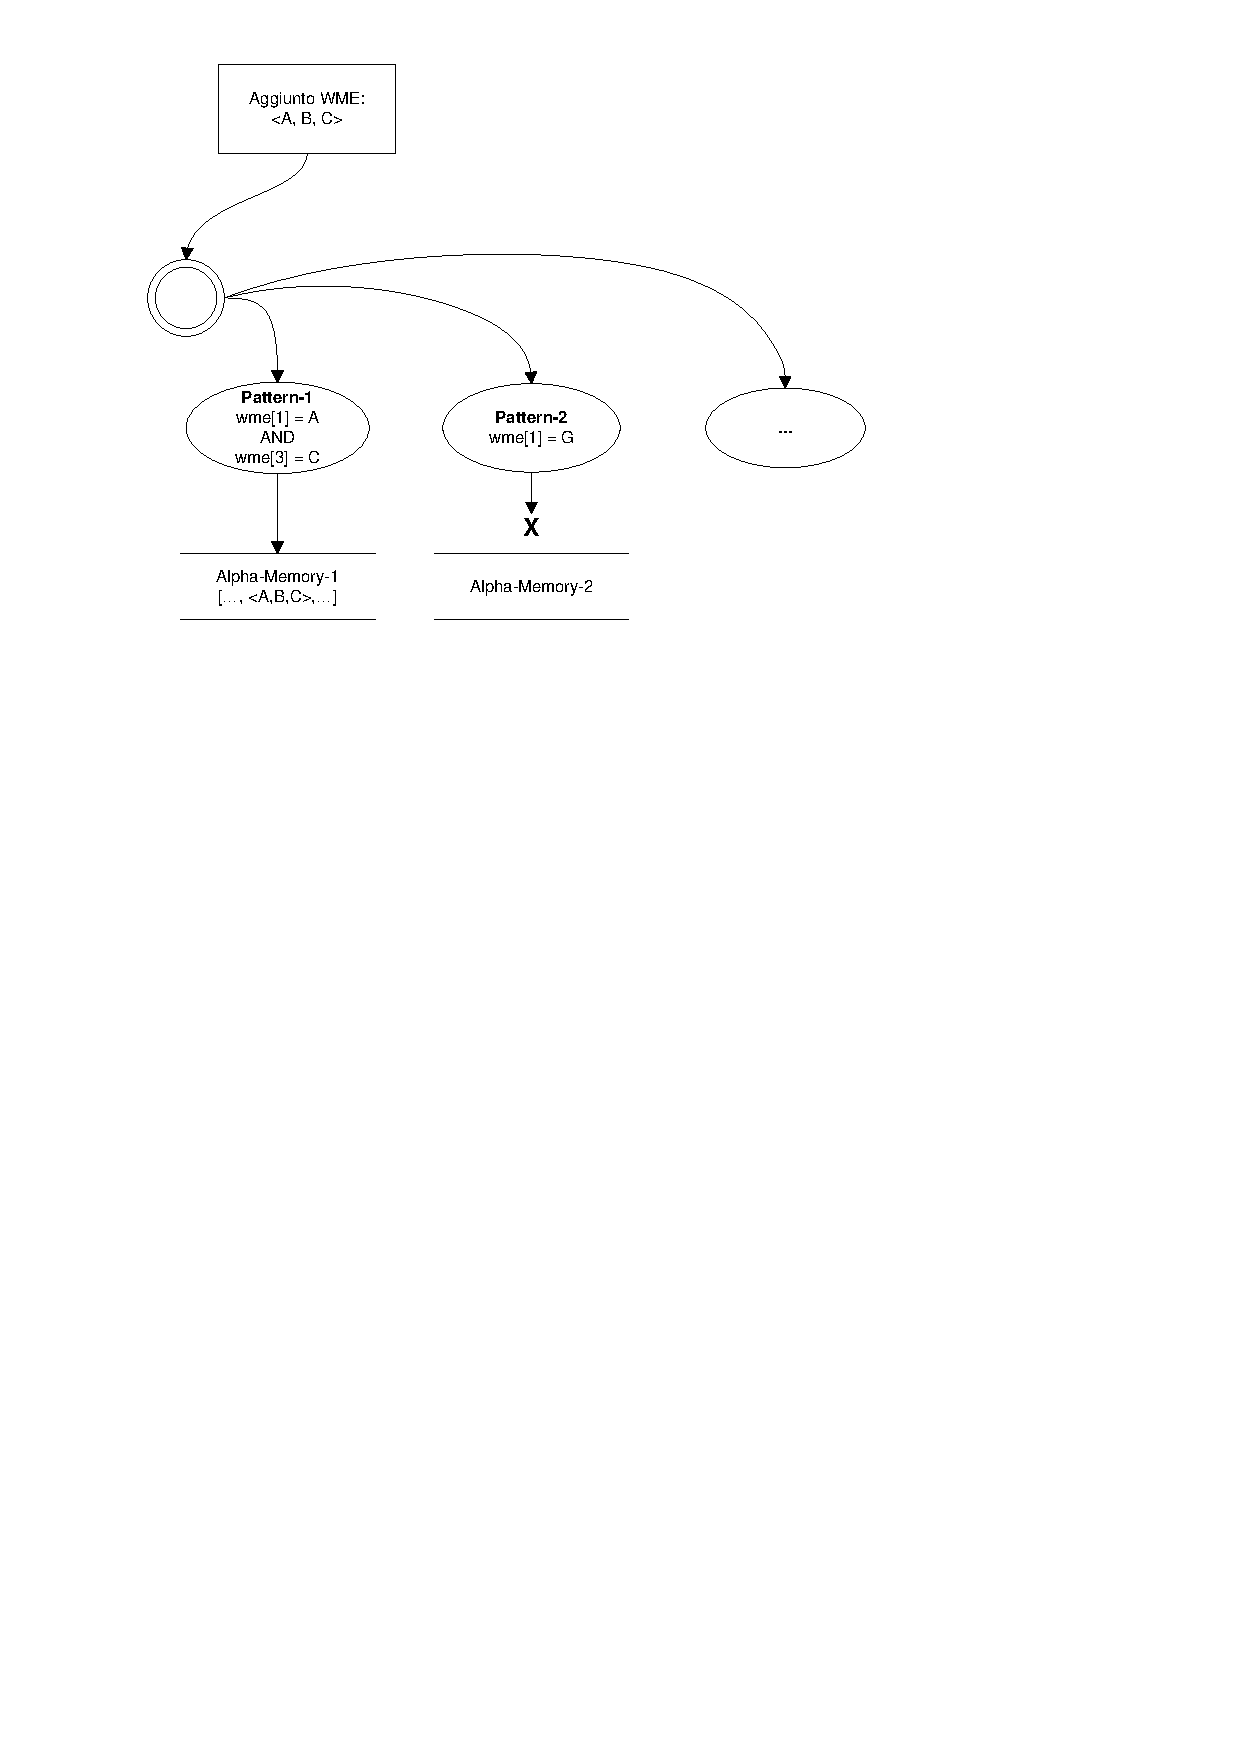
\includegraphics[viewport=70 545 416 812]{Immagini/Capitolo1/Asserzione.pdf}
\caption{Asserzione di un nuovo elemento della \emph{working memory} e valutazione tramite algoritmo RETE}\label{fig:asserzione}
\end{figure}

Quando un nuovo elemento viene asserito (\figurename~\ref{fig:asserzione}), e quindi entra a far parte della descrizione dello stato fornita dalla \emph{working memory}, l'algoritmo esegue una valutazione di ogni pattern singolarmente per il nuovo elemento aggiunto, e solo in caso di verifica positiva l'elemento stesso viene inserito all'interno dell'unità di memoria locale~\cite{forgy1982}.

Quando un elemento fuoriesce dalla \emph{working memory}, lo stesso viene rimosso da tutte le unità di memoria locali dei pattern in cui l'elemento è memorizzato. Il processo di ricerca può avvenire ripetendo nuovamente le verifiche per i singoli pattern~\cite{forgy1982} oppure, più efficientemente, tenendo in una porzione di memoria separata una lista di collegamenti fra elementi e le memorie in cui essi sono contenuti.~\cite{Doorenbos95productionmatching}

La scansione dell'intero \emph{rules-set} viene evitata attraverso l'utilizzo di una struttura a grafo per la rappresentazione delle regole. In seguito ad una fase di compilazione (\figurename~\ref{fig:grafo-regola}), la porzione \emph{LHS} delle regole viene scomposta nei singoli pattern. Per ognuno di essi viene realizzata, qualora non fosse possibile condividere una struttura analoga creata precedentemente, un circuito di nodi in grado di eseguire dei test su singoli elementi della \emph{working memory}. Come ultimo elemento del circuito viene aggiunta un'unità di memoria locale, denominata \emph{Alpha-Memory}, la quale accoglierà l'insieme di elementi che, singolarmente, hanno verificato l'elenco di condizioni che il circuito descrive~\cite{Doorenbos95productionmatching}.
L'insieme di circuiti derivanti dalla compilazione dei singoli pattern prende il nome di \emph{Alpha-Network}.

Una seconda porzione della rete è quella nota con il nome di \emph{Beta-Network}. In questa sezione vengono eseguiti i test di coerenza sul binding delle variabili fra le condizioni. Durante la fase di compilazione, una volta create le porzioni \emph{alpha} di ogni singolo pattern, quelli appartenenti alla stessa \emph{LSH} vengono collegati fra loro attraverso l'uso di speciali nodi, chiamati \emph{Join-Node}. Questi nodi, oltre a riunire singoli pattern in una catena che rappresenti l'intera \emph{LHS}, hanno il compito di eseguire l'insieme di test necessari alle verifiche di coerenza sul valore delle variabili, dove necessario. Qualora i test eseguiti in questi nodi a due input risultassero positivi, verrebbe creata una struttura contenente i due elementi della memoria di lavoro che sono risultati coerenti e la stessa memorizzata all'interno di una unità di memoria agganciata direttamente al \emph{Join-Node}. 
La struttura prende il nome di \emph{Token}\footnote{Nella formulazione dell'algoritmo proposto originariamente in \cite{forgy1979} e \cite{forgy1982} con il termine \emph{Token} si faceva riferimento a una descrizione di un cambiamento nella \emph{working memory}, notificato ai nodi componenti la rete tramite l'uso di \emph{tag}. La formulazione proposta in \cite{Doorenbos95productionmatching} utilizza l'appellativo per indicare una sequenza di \emph{working memory elements} che abbiano verificato una porzione della \emph{beta-network}. Il concetto di tag, usati nella prima formulazione per indicare il tipo di modifica che il \emph{token} rappresentava, nella seconda formulazione è completamente assente}.

\begin{figure}
\centering
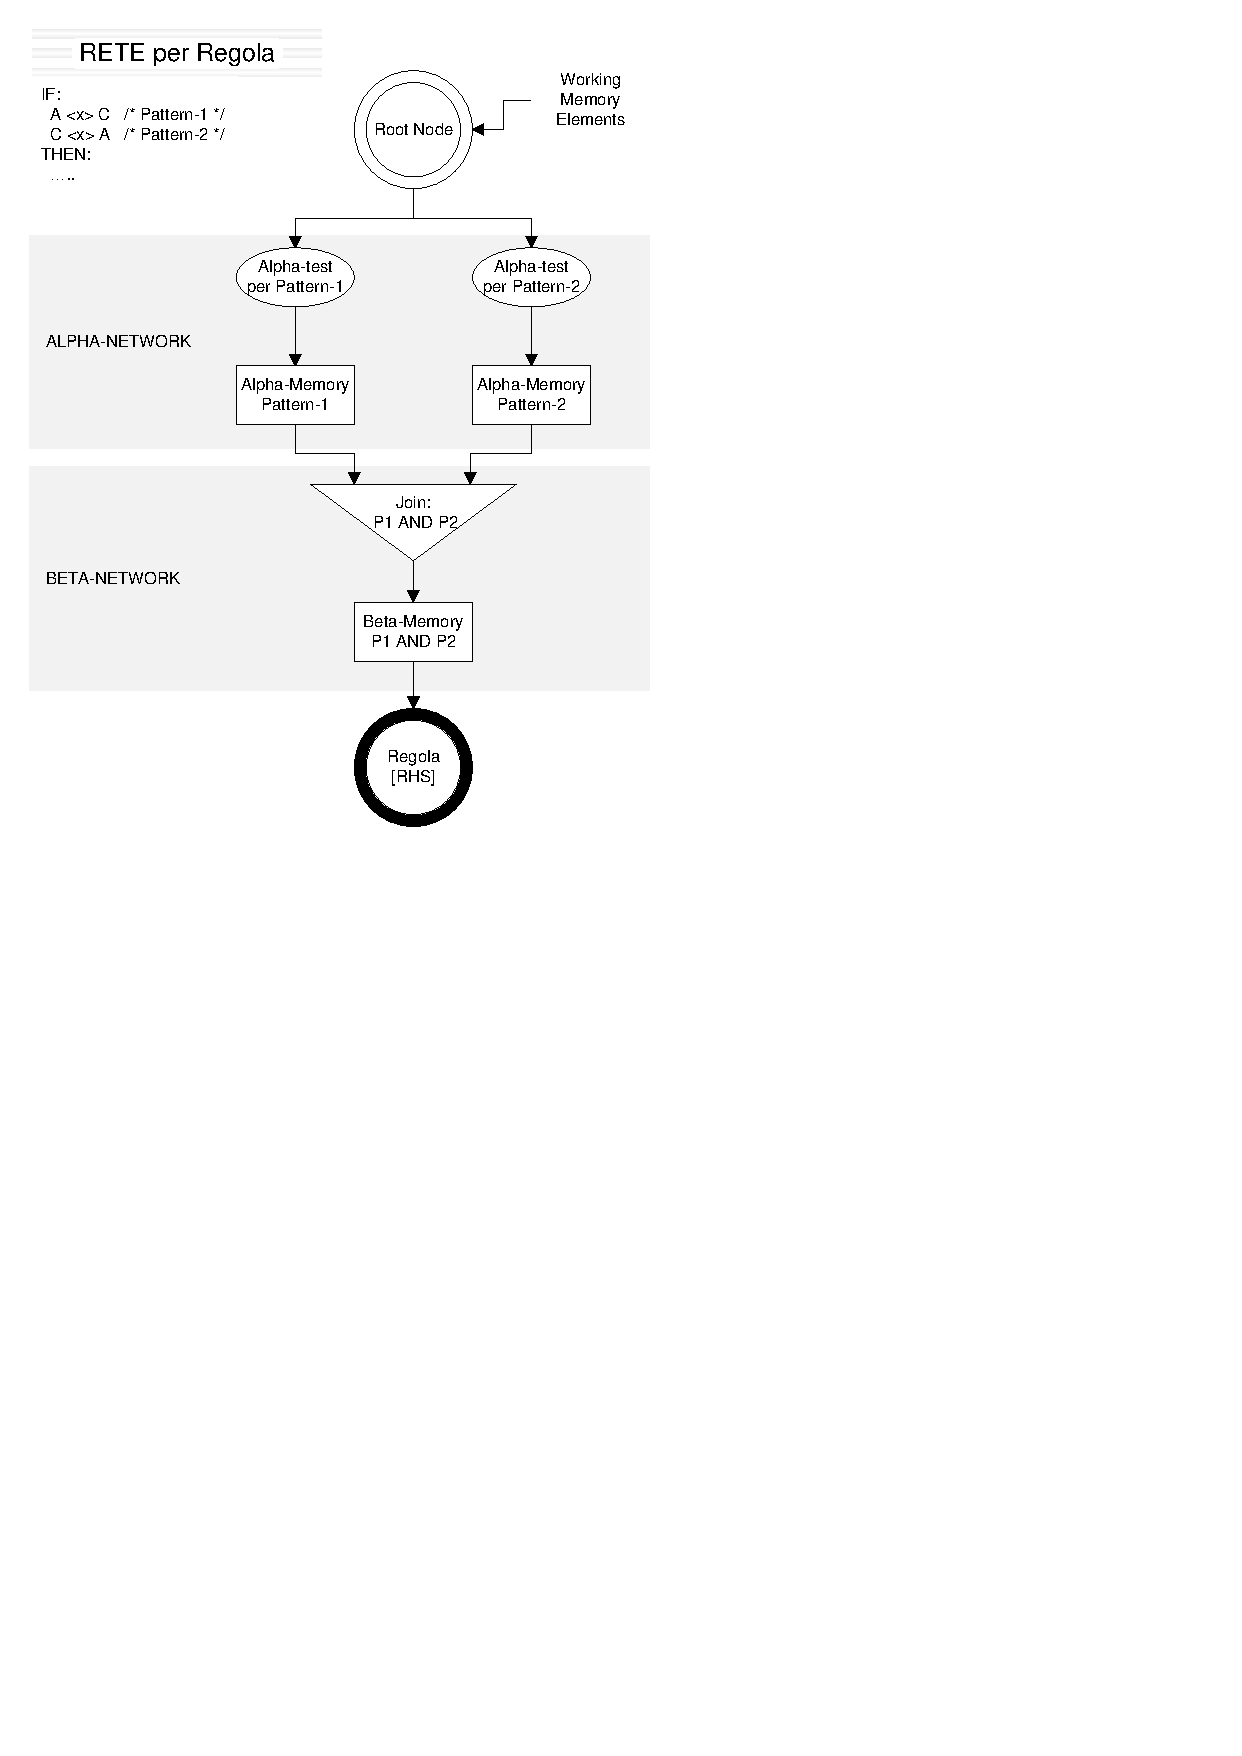
\includegraphics[viewport=14 446 312 829]{Immagini/Capitolo1/RETE-Regola.pdf}
\caption[Grafo esplicito di RETE per una regola]{Rappresentazione esplicita del grafo ottenuto dalla compilazione di una regola: vengono creati circuiti alpha per ogni \emph{pattern} e in seguito congiunti valutando la coerenza del valore della variabile $x$ fra i riscontri.}\label{fig:grafo-regola}
\end{figure}

L'utilizzo di un ulteriore tipo di memoria nella \emph{Beta-Network}, chiamata \emph{Beta-Memory}, consente di memorizzare attivazioni parziali che risultano valide solo per una porzione della regola, in attesa, che tramite l'asserzione di ulteriori fatti, l'intera regola risulti attivabile.

Il processo di trasformazione delle regole porta a due benefici sostanziali:
\begin{itemize}
	\item la compilazione dei singoli pattern eseguita per la formazione dell'\emph{alpha-network} consente di partizionare la working-memory in frammenti di minori dimensioni. Questo si traduce in un minor numero di confronti durante i test di coerenza. Inoltre, pattern simili presenti in più regole vengono accorpati e rappresentati da un unico circuito \emph{alpha}. La fase di valutazione verrà eseguita soltanto una volta per tipo di pattern.
	\item gruppi di pattern simili, analogamente a quanto descritto nel punto precedente, vengono accorpati in un solo circuito \emph{beta}, riducendo ulteriormente i costi delle verifiche per i test di coerenza.
\end{itemize}

Il processo di creazione della rete può avvenire attraverso un reale processo di compilazione \cite{forgy1982} che prevede la conversione dell'intero \emph{rules-set} in una sequenza di istruzioni ed espressioni che rappresentino le varie condizioni (implementazione \emph{compilata}), oppure attraverso un processo di creazione di una rappresentazione esplicita di grafo nelle modalità citate poc'anzi (implementazione \emph{interpretata}). 

Il vantaggio della prima variante è la maggiore velocità, che contrasta tuttavia con un maggior consumo di memoria e maggiore difficoltà di implementare procedure che, attraverso l'aggiunta o la rimozione di produzioni durante l'esecuzione, siano in grado di alterare la struttura della rete~\cite{Doorenbos95productionmatching}.
La seconda variante rende più semplice l'implementazione di procedure di manipolazione della rete e risulta globalmente di più facile implementazione e comprensione. Purtroppo questi vantaggi prevedono uno scambio di tipo prestazionale~\cite{Doorenbos95productionmatching}.

\section{Strumenti di sviluppo}

%%%%%%%%%%%%% VALUTARE RIORGANIZZAZIONE %%%%%%%%%%%%%%%%%

Tutti gli strumenti di sviluppo per sistemi esperti sono orientati a supportare la creazione di \emph{prototipi}. Un prototipo rappresenta un modello funzionante le cui funzionalità sono equivalenti ad una porzione ridotta di quelle del prodotto finale~\cite{jackson1999}.
L'idea è quella di sviluppare, nelle prime fasi del progetto, dei ''\emph{proof of concept}'' che possano essere valutati e criticati da esperti e utenti e che siano in grado di risolvere parti del problema. Questa attività è utilizzata soprattutto come un'opportunità per definire meglio requisiti e individuare criticità, verificando inoltre l'effettiva trattabilità di problematiche prima di effettuare investimenti eccessivi.

Una possibilità è che gli artefatti prodotti vengano quindi scartati al termine delle valutazioni, ma gli approcci verificati con la produzione dei prototipi stessi vengono conservati e riapplicati durante la fare di sviluppo reale del prodotto. Altre modalità prevedono l'accorpamento e sviluppo incrementale delle funzionalità del prodotto finale tramite fasi reiterate di produzione di \emph{protitipi} e valutazione.

Il numero di ambienti di sviluppo per sistemi esperti è cresciuto negli anni e con esso il numero e la tipologia di funzionalità offerte.
L'evoluzione di questi sistemi è stata motivata con il tempo e la quantità di sforzo richiesto per la costruzione di sistemi esperti.

Lo sviluppo si è focalizzato in molte aree di interesse, spaziando dall'ambito delle modalità di rappresentazione della conoscenza a quello dei meccanismi di inferenza, dallo sviluppo di regimi di controllo alla ricerca nell'ambito dei linguaggi di specifica. Indipendentemente dalle modalità con le quali è stato tentato il miglioramento, lo slancio evolutivo era ad ogni modo focalizzato nell'ambito di:
\begin{itemize}
	\item ridurre tempi e costi di sviluppo dei sistemi esperti
	\item migliorare l'affidabilità e la qualità generale dei sistemi prodotti
	\item focalizzare le attività delle varie figure professionali interessate nello sviluppo negli ambiti di propria competenza.
	\item separare le attività di analisi della conoscenza da quelle legate allo sviluppo del prodotto.
	\item fornire strumenti per velocizzare e migliorare le attività di acquisizione e aggiornamento della conoscenza.
\end{itemize}

I miglioramenti hanno incrementato in questo modo le possibilità di successo nello sviluppo di sistemi esperti. Come ulteriore effetto, il ridursi della complessità generale delle operazioni di realizzazione ha consentito di gestire e produrre soluzioni di sempre maggiore complessità.

\subsection{L'evoluzione degli strumenti di sviluppo}

Tornando indietro agli albori della produzione di sistemi esperti, i meccanismi di inferenza e le basi di conoscenza erano accoppiati fra loro. La prima generazione di sistemi non erano altro che grandi applicazioni scritte in linguaggi come LISP~\cite{knowbel1993}.

Nonostante tutti i linguaggi di programmazione potessero essere utilizzati per la produzione di sistemi esperti, alcuni di essi offrivano caratteristiche che rendevano tale attività più agevole. Rientrano in questa categoria linguaggi largamente utilizzati nelle prime fasi come il LISP e Prolog.
Purtroppo, la quantità di tempo e sforzo richiesto per la produzione usando queste tipologie di linguaggi diventava rapidamente insostenibile con l'aumentare della complessità. Inoltre, l'accoppiamento fra le funzionalità necessarie all'inferenza e quelle per la rappresentazione e la gestione della conoscenza non permetteva una distinzione di ruoli fra gli ingegneri di sistema e quelli della conoscenza~\cite{development1993}.

Questo approccio alla lavorazione venne superato nella successiva generazione. Durante la creazione di sistemi di seconda generazione come MYCIN, i ricercatori si accorsero dell'importanza di implementare i sistemi in modo che fosse possibile una separazione fra la base di conoscenza e i meccanismi che realizzavano il ragionamento.

Rimuovendo la conoscenza di dominio da questi sistemi vennero realizzati i primi sistemi di tipo \emph{Skeletal Shell}: utilizzando gli strumenti sviluppati nel progetto originale e inserendo nuova conoscenza di dominio era possibile creare una grande verità di nuovi sistemi esperti con un sforzo relativamente ridotto. I sistemi di seconda generazione di maggior successo hanno dato vita a \emph{Shell} per lo sviluppo di sistemi esperti. Ne sono esempi EMYCIN, KAS e EXPERT: rispettivamente prodotti rimuovendo le conoscenze di dominio da MYCIN, PROSPECTOR e CASNET.
Sebbene l'utilizzo di questi strumenti velocizzasse la produzione di nuovi sistemi di diversi ordini di grandezza, la necessità di attenersi alle strategie utilizzate nei sistemi originali rappresentava un limite alla flessibilità del sistema ed ai possibili ambiti di utilizzo (\figurename~\ref{fig:classificazione-tools}). 

\begin{figure}
\centering
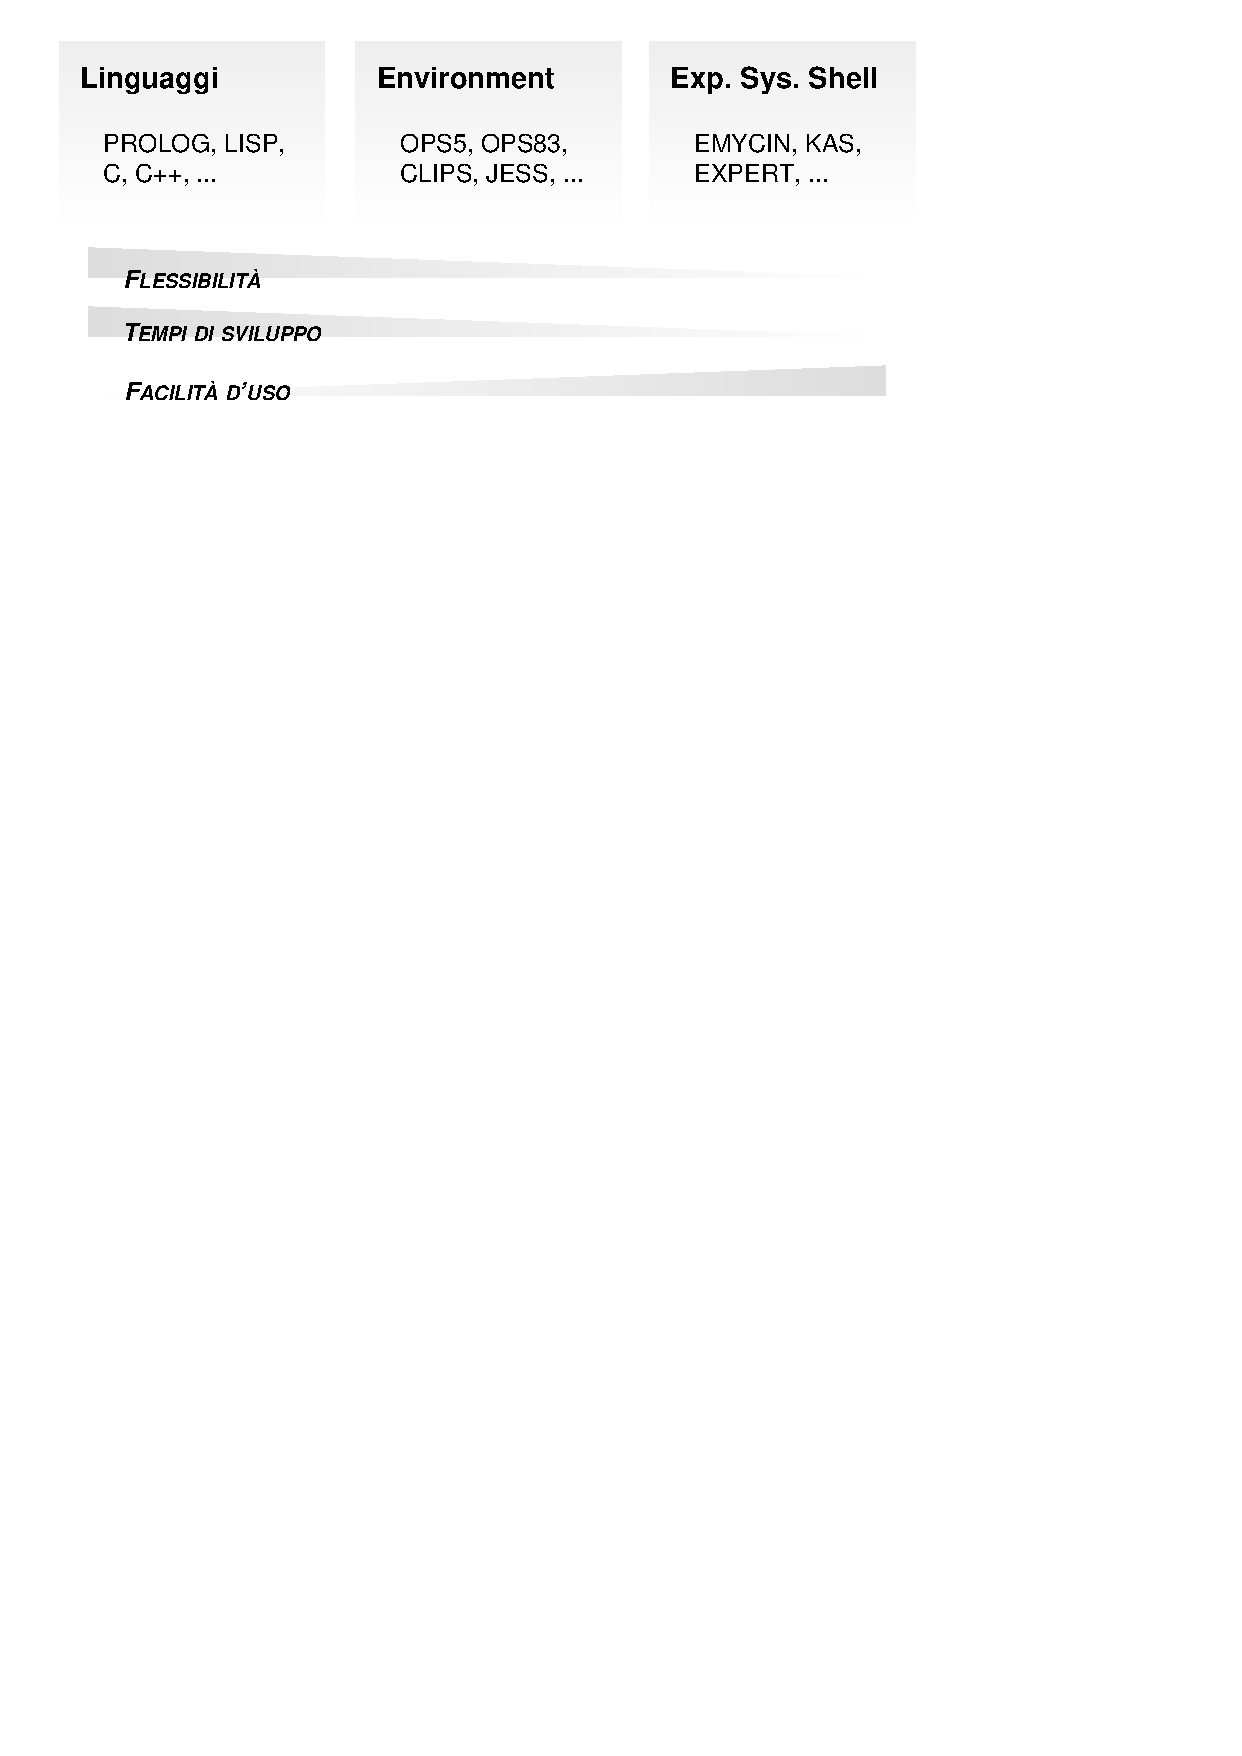
\includegraphics[width=0.9\textwidth, viewport=28 650 440 824]{Immagini/Capitolo1/Classificazione-tools.pdf}
\caption{Classificazione degli strumenti di sviluppo per sistemi esperti}\label{fig:classificazione-tools}
\end{figure}

Il successivo passo evolutivo fu compiuto con l'introduzione di linguaggi di alto livello orientati alla realizzazione di sistemi esperti e gli ambienti di programmazione multi-paradigmatici.
I primi, introdotti nella seconda metà degli anni '70, consentivano grande flessibilità e permettevano di svolgere attività di prototipazione rapida. Queste caratteristiche si traducevano nella possibilità di sperimentare  e valutare soluzioni progettuali con costi e tempi relativamente contenuti. Inoltre, per la natura stessa degli strumenti, il codice prodotto poteva essere testato in maniera incrementale durante la scrittura (possibilità offerta dal fatto che le interfacce \emph{runtime} e \emph{buildtime} erano prossime fra loro)~\cite{jackson1999}.

Spesso, questo tipo di \emph{shell} limitava la propria offerta ad un particolare tipo di formalismo per la rappresentazione della conoscenza oppure un particolare regime di controllo. La flessibilità offerta dai linguaggi di alto livello risiedeva proprio nella possibilità, per il progettista, di accedere ad approcci differenti e in questo modo spaziare fra meccanismi multipli.

Gli ambienti di programmazione multi-paradigmatici o \emph{Expert System Environment} accoppiavano la filosofia alla base dei linguaggi di alto livello con la possibilità di usufruire di differenti modalità di rappresentazione della conoscenza, regimi di controllo e paradigmi di programmazione in base alle esigenze.
Questo genere di strumenti permetteva ai programmatori di selezionare e combinare differenti moduli software. In assenza di un singolo linguaggio di rappresentazione della conoscenza che fosse valido per ogni applicazione, la soluzione era quella di fornire e rendere disponibile più di uno schema contemporaneamente.

\begin{quote}
''Sebbene non ci sia una teoria ben articolata sui sistemi basati su approccio ibrido, l'esperienza con schemi di rappresentazione e inferenza differenti ha mostrato che ognuno ha le sue debolezze; quindi la strategia di miscelare gli schemi tenta di giocare il più possibile con i loro punti di forza.''~\cite{jackson1999}
\end{quote}

\begin{figure}[h]
\centering
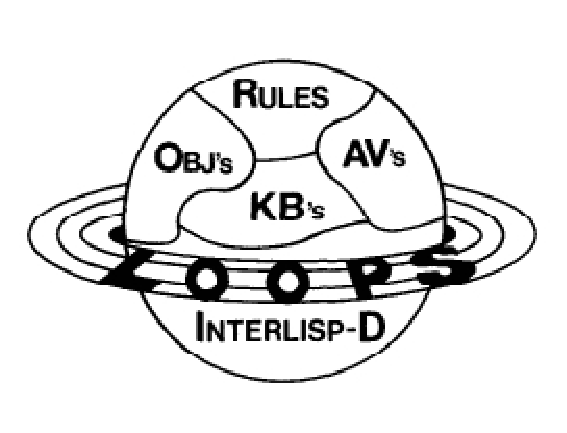
\includegraphics[scale=0.7, viewport=0 0 272 184]{Immagini/Capitolo1/LOOPS-logo.pdf}
\caption[Il logo di LOOPS]{Il logo di LOOPS: illustra i differenti paradigmi disponibili nell'\emph{environment}. Immagine originale tratta da~\cite{loops1983aaai}.}\label{fig:logo-LOOPS}
\end{figure}

Il primo esempio di ambiente multi-paradigmatico a quattro schemi fu LOOPS~(1983, \figurename~\ref{fig:logo-LOOPS}): fondeva insieme quattro paradigmi di programmazione (procedurale, basata su regole, orientata agli oggetti, orientata ai dati) all'interno di un'architettura basata sullo scambio di messaggi~\cite{loops1983aaai}.

\subsection{Skeletal Shell}
Le \emph{Shell} avevano l'obiettivo di consentire, anche a persone senza una esperienza specifica di programmazione tradizionale, di utilizzare gli sforzi compiuti da altri nell'ambito della soluzione di problematiche simili.
Fu chiaro però che l'applicabilità dell'architettura di base non era di tipo universale, sebbene consentisse di realizzare sistemi in ambiti simili a quelli per il quale il progetto era concepito.

\begin{quotation}
''EMYCIN è progettato per aiutare la costruzione e l'esecuzione di programmi che forniscono consigli. [$\dots$]

EMYCIN non è progettato per essere un linguaggio di rappresentazione \emph{general-purpose}. \`E completamente inadatto per alcuni problemi. Le limitazioni derivano in gran parte dal fatto che EMYCIN ha scelto un solo metodo per rappresentazione della conoscenza che fosse basilare, semplice da leggere e interpretare: regole di produzione applicate tramite un regime di controllo basato sul \emph{backward-chaining}~[$\dots$]''~\cite{puff1982}
\end{quotation}

Un esempio risiede in EMYCIN: sebbene consentisse di utilizzare l'architettura alla base di MYCIN e applicarla anche ad altri domini specifici nell'ambito medico (PUFF~\cite{puff1982}) o in altri ambiti (SACON~\cite{bennett1979}), la sua architettura non era abbastanza generalizzata per essere definita \emph{general-purpose}~\cite{vanmelle1984}. Era tuttavia valido per sviluppare sistemi basati sull'uso di un approccio deduttivo a problemi diagnostici, dove è disponibile una grande quantità di conoscenza ed è possibile individuare e definire le categorie diagnostiche in anticipo.

A discapito dei vantaggi in termini di semplicità nella rappresentazione della conoscenza e della specifica del sistema offerti dai tool di tipo \emph{Skeletal Shell}, le più grandi critiche a questa classe di sistemi risiedono in tre punti principali~\cite{Aikins1983163}:

\begin{itemize}
	\item[(1)] Il formalismo basato solo su regole, che la grande maggioranza di questa classe di sistemi offriva, rendeva difficile la distinzione fra conoscenza di tipo euristico, quella di controllo e quella adibita alla valutazione dei parametri richiesti. Questa limitazione rendeva difficile la comprensione dei sistemi.
	\item[(2)] L'aggiornamento e l'aggiunta di nuova conoscenza in questi sistemi rendeva difficile effettuare previsioni sull'impatto che le modifiche avrebbero avuto sul sistema nella sua interezza.
	\item[(3)] La scelta di un preciso regime di controllo spesso si adattava bene ad alcune attività, mentre rendeva difficoltoso lo sviluppo di componenti differenti dello stesso sistema (ad esempio, il regime basato su \emph{backward-chaining} offerto da EMYCIN rendeva da una parte agevole il processo di diagnosi, ma dall'altra ardua la realizzazione delle dinamiche di spiegazione).
\end{itemize}

\subsection{Expert System Environment}
Le \emph{Shell} di tipo \emph{general-purpose} offrono un maggiore controllo e flessibilità rispetto alle \emph{Skeletal Shell} rimuovendo diversi vincoli, ma questa ritrovata flessibilità viene pagata con maggiori oneri a carico dei progettisti. 

Strumenti dotati di maggiore flessibilità offrivano solo meccanismi di rappresentazione e \emph{problem-solving} basilari. Questo li rendeva adatti a qualsiasi ambito e problematica, ma il basso livello di sofisticazione obbligava gli ingegneri della conoscenza a specificare personalmente parte dei meccanismi di ragionamento e di rappresentazione. Esempi di questa sottoclasse di strumenti sono ROSIE, OPS5 e Prolog\footnote{Sebbene il Prolog sia un linguaggio di programmazione logica general-purpose, la disponibilità di meccanismi di ragionamento basilari basati su un regime di tipo \emph{backward-chaining} e la forma dichiarativa del linguaggio che rende agevole la rappresentazione della conoscenza lo rendono ascrivibile anche alla categoria delle \emph{General-Purpose Shell}}.

Maggiore semplicità era quella offerta invece dai sistemi come BLOBS, G2 o CubiCal~\cite{development1993}. Il loro ambito di utilizzo veniva ridotto, ma il maggiore livello di sofisticazione nelle forme ragionamento, unito alla disponibilità di paradigmi multipli per la rappresentazione della conoscenza, rendeva più agevole lo sviluppo di sistemi esperti. Inoltre agli ingegneri della conoscenza era richiesta una minore conoscenza delle dinamiche del sistema di base. La modifica dei meccanismi di ragionamento era ancora possibile, anche se non obbligatoria.

Gli strumenti posti al più alto grado di sofisticazione nella categoria degli \emph{environment} erano progettati per affrontare più aree di problemi. Offrivano paradigmi multipli per la specifica della conoscenza e del ragionamento, uniti a caratteristiche e utilità orientate allo sviluppo dei sistemi esperti ed alla riduzione dei tempi di iterazione nei processi di prototipazione. 

La presenza di interpreti già integrati e di paradigmi multipli di rappresentazione rendevano estremamente ridotto il carico degli ingegneri della conoscenza nella definizione dei nuovi sistemi. Nonostante tutto, la scelta di utilizzare alcune di queste funzionalità portava ad influenzare fortemente il design nei casi in cui i paradigmi offerti non corrispondessero perfettamente ai requisiti~\cite{development1993}.

\subsubsection[ART]{ART (Automated Reasoning Tool)}
ART è uno dei primi strumenti di sviluppo per sistemi esperti scritti in LISP. Offriva strutture come oggetti, regole di produzione, meccanismi per il mantenimento della catena di verità ed integrava un paradigma di programmazione orientato agli oggetti~\cite{art1998}.

\subsubsection[ART-IM]{ART-IM (ART for Information Management)}
ART-IM è una re-implementazione del sistema ART in linguaggio C, basato su una versione proprietaria dell'algoritmo RETE per la realizzazione di un regime di tipo \emph{forward-chaining} e un meccanismo di mantenimento della verità (già presente in ART).

Nonostante l'implementazione fosse fortemente incentrata sul motore inferenziale di tipo \emph{forward}, il sistema permetteva anche ragionamento basato sulla concatenazione all'indietro. L'utilizzo del regime alternativo era però sottoposto alla necessità di una specifica esplicita di strutture di controllo, alla definizione di priorità e obiettivi.

Una caratteristica importante introdotta nella re-implementazione in C era la possibilità di integrare funzionalità aggiuntive tramite lo sviluppo di funzioni separate, sempre in linguaggio C, ed integrabili durante la compilazione del sistema.

L'utilizzo di questa caratteristica ha permesso la realizzazione di ulteriori varianti (come ART-Ada~\cite{artadanasa1990}, per l'utilizzo nella specifica dei sistemi tramite linguaggio ADA), rese disponibili in seguito.

La grande varietà di funzionalità e le potenzialità offerte dal sistema nella sua interezza lo rendevano però uno strumento non adatto a progettisti alle prime armi: era richiesta conoscenza dei linguaggi C e LISP oltre che del paradigma di sviluppo orientato agli oggetti~\cite{development1993}.

\subsubsection[CLIPS]{CLIPS (C Language Integrated Production System)}

CLIPS è un \emph{environment} sviluppato al NASA Johnson Space Center nella metà del 1980. Prende spunto da tool come OPS5 e ART, supportandone le caratteristiche di maggior importanza e introducendone di nuove come le funzionalità relative alla programmazione procedurale. 

La sintassi utilizzata per lo sviluppo dei sistemi esperti è simile a quella del linguaggio LISP. 

Lo sviluppo iniziò in un contesto in cui erano emergenti, ma ancora costose, soluzioni di environment basati su linguaggio C. Il risultato è il sistema meno costoso e di maggiore reperibilità al mondo, non meno efficiente di soluzioni commerciali. La prima versione non integrava funzionalità chiave introdotte solo successivamente, come il linguaggio procedurale e il paradigma di programmazione ad oggetti~\cite{jackson1999}.

Il sistema è liberamente utilizzabile per uso personale ed accademico, mentre l'uso commerciale è soggetto all'acquisto di una licenza personale \emph{una tantum}.

Lo sviluppo del progetto, attualmente affidato ad una sola persona, è ancora in atto. Il codice sorgente è disponibile pubblicamente, cosi come le versioni compilate.

Le prime versioni di CLIPS (poco più che prototipi, implementazioni \emph{clean-room} di caratteristiche di ART)~\cite{clipsarch1992}, utilizzavano un motore basato su una implementazione dell'algoritmo RETE con regime \emph{forward-chaining} e specifica nella forma di regole di produzione. 

Il successo del progetto prima come \emph{training-tool}, poi come reale ambiente di sviluppo e distribuzione di sistemi esperti, ha giustificato lo sviluppo di versioni successive. Il progetto è stato esteso con l'integrazione del paradigma procedurale e ad oggetti (COOL).

Il successo di CLIPS è attestato dal grande numero utilizzatori: una stima realizzata nel 1992 indicava che fosse superiore a 3000, senza contare l'adozione all'interno del laboratori NASA, l'utilizzo in ambito militare, governativo, accademico e commerciale\footnote{Il numero di download del sistema dalla piattaforma di distribuzione ufficiale negli ultimi 4 anni ha superato quota 200.000. Non sono presenti misurazioni nel periodo precedente al Gennaio 2008.}~\cite{clipsarch1992}.

Negli anni sono state derivate dal progetto originale diverse varianti che espandevano specifiche categorie di caratteristiche. Alcuni esempi sono ECLiPSe~\cite{haley1991}, eCLIPS~\cite{eclips} e FuzzyCLIPS~\cite{fuzzyclips}.

\subsubsection[JESS]{JESS (Java Expert System Shell)}
Nato originariamente come un clone di CLIPS, JESS è un \emph{environment} completamente scritto in Java con l'obiettivo di integrare le funzionalità offerte da CLIPS con tecnologie per il web basate su Java. 
Le prime versioni offrivano il supporto ad un set limitato delle caratteristiche di CLIPS. Con il tempo lo sviluppo si è diretto verso l'aggiunta di funzionalità originali in maniera indipendente dal progetto padre, separando in questo modo i due progetti~\cite{laerhoven1999}~\cite{jessfaq}~\cite{jessmanual}.

Sebbene JESS non integri un linguaggio di specifica di tipo \emph{object-oriented}, la forte integrazione con il linguaggio Java con cui è implementato consente di utilizzare particolari notazioni, gli \emph{shadow-fact}, per collegare elementi nella \emph{working-memory} con istanze di classi specificate in linguaggio Java.


\subsection{Il problema dell'integrazione}

Molti degli strumenti originariamente progettati per lo sviluppo di sistemi esperti stand-alone non supportavano l'integrazione con altri componenti software di utilizzo comune come database o fogli di calcolo.
A volte i linguaggi, o le piattaforme, scelti per l'implementazione di questi sistemi erano un freno alle possibilità di integrazione. I primi strumenti basati sul linguaggio LISP richiedevano apparecchiature appositamente sviluppate (\emph{LISP-machines}) e grandi quantitativi di memoria. Questo si traduceva, oltre che nella richiesta di grandi investimenti, anche in architetture fortemente specializzate. Il grande costo di queste apparecchiature limitava anche le possibilità di diffusione e successo dei prodotti sviluppati con questi tool~\cite{development1993}.
Questi strumenti basati su LISP introducevano anche grossi problemi in termini di portabilità degli artefatti prodotti~\cite{clipsarch1992}.

Per superare questi ostacoli, molti dei tool originariamente sviluppati in LISP vennero con il tempo riscritti per essere utilizzati su piattaforme emergenti di più grande diffusione (come le workstation e le piattaforme convenzionali che utilizzavano Unix come sistema operativo prima, o i Personal Computer poi).
Durante questo processo di conversione, la scelta di molti ricadde verso il linguaggio C, molto diffuso e supportato da tutte le piattaforme. L'adozione del C portò ad un incremento prestazionale dei sistemi oltre ad offrire nuovi scenari in cui sperimentare l'integrazione fra il software disponibile sulle nuove piattaforme e gli strumenti di sviluppo per sistemi esperti.
Prendendo in esame CLIPS, il sistema poteva essere integrato all'interno di qualsiasi applicazione che fosse in grado di interfacciarsi direttamente con librerie scritte in linguaggio C. JESS estende ulteriormente queste possibilità tramite l'utilizzo di Java, linguaggio emergente negli ultimi anni sia in ambiente \emph{coorporate} che nei prodotti di largo consumo.

Studi effettuati negli ultimi anni hanno analizzato l'efficienza, la facilità e le possibilità offerte dallo sviluppo di software con vari linguaggi di programmazione~\cite{naiditch1999}~\cite{Zeigler_95}~\cite{prechelt2000}~\cite{prashant2008}.
Sebbene questi studi abbiamo mostrato, come prevedibile, che le caratteristiche di particolari linguaggi si adattino meglio ad alcuni ambiti di utilizzo rispetto che ad altri, un elemento comune emerso riguarda l'impatto che la scelta del linguaggio ha sui costi di sviluppo e l'affidabilità degli artefatti prodotti. Nonostante la grande flessibilità offerta dal linguaggio C, i costi affrontati per lo sviluppo, il testing e la manutenzione degli artefatti prodotti erano superiori rispetto a quelli imposti da altri linguaggi come Ada~\cite{Zeigler_95}, Java~\cite{prashant2008} o a linguaggi interpretati come Perl o Python\cite{prechelt2000}.

\section{Obiettivi di questa tesi}
Negli ultimi anni Internet, e più specificamente il \emph{World Wide Web}, sta evolvendo da un medium per lo scambio di informazioni verso una piattaforma onnipresente per la distribuzione di qualsiasi genere di servizi come \emph{Web banking}, \emph{E-Commerce}, \emph{E-Government}, etc. La ragione alla base di questa rapida evoluzione del Web è il grande numero di possibilità che questa forma di distribuzione offre, unito al grande successo che questo genere di soluzioni sta riscontrando verso l'utenza.

L'orientamento verso il calcolo distribuito, lo stoccaggio di dati personali tramite servizi \emph{cloud-based}, la conversione del consumo classico verso declinazioni digitali, sono tutti frammenti di questa evoluzione.

In questo ambito, la possibilità di integrazione delle tecnologie classiche per la realizzazione di sistemi esperti con strumenti di nuova generazione orientati allo sviluppo per il web offre molti spunti per la ricerca nell'ambito degli \emph{expert system environment}. L'approfondimento delle tematiche relative allo sviluppo di nuove soluzioni rappresenta uno spunto per capire in maniera più intima le dinamiche alla base del funzionamento dei sistemi esperti e degli strumenti che ne consentono la creazione e la distribuzione.

%Unire problematiche tanto differenti all'interno di un solo strumento richiede la progettazione di soluzioni flessibili.

%%%%%%%%%%%% UNIRE UN CAPOVERSO PER INDICARE I FINI DIDATTICI %%%%%%%%%%%%%%%

Lo scenario di riferimento descritto nell'arco di questo capitolo, unito alle problematiche emergenti dallo sviluppo orientato al Web, è la base su cui si vuole proporre un \emph{environment per sistemi esperti} flessibile e che consenta un'integrazione rapida con tecnologie esistenti orientate al web.

Gli obiettivi perseguiti nell'ambito di questa tesi sono riassumibili come segue:
\begin{itemize}
	\item fornire un \emph{expert system environment} dotato di una architettura flessibile in grado di permettere l'aggiunta di nuove caratteristiche;
	\item estendere il sistema prodotto con funzionalità che consentano la distribuzione dei servizi offerti dall'\emph{environment} anche attraverso un modello d'architettura di tipo \emph{client-server}, che agevoli la creazione di soluzioni basate su calcolo distribuito.
\end{itemize}




\appendix
\addcontentsline{toc}{chapter}{\bibname}
\onehalfspacing
\printbibliography

\end{document}
